
%% 
%% Copyright 2007, 2008, 2009 Elsevier Ltd
%% 
%% This file is part of the 'Elsarticle Bundle'.
%% ---------------------------------------------
%% 
%% It may be distributed under the conditions of the LaTeX Project Public
%% License, either version 1.2 of this license or (at your option) any
%% later version.  The latest version of this license is in
%%    http://www.latex-project.org/lppl.txt
%% and version 1.2 or later is part of all distributions of LaTeX
%% version 1999/12/01 or later.
%% 
%% The list of all files belonging to the 'Elsarticle Bundle' is
%% given in the file `manifest.txt'.
%% 
%% Template article for Elsevier's document class `elsarticle'
%% with harvard style bibliographic references
%% SP 2008/03/01

\documentclass[preprint,12pt,authoryear]{elsarticle}

%% Use the option review to obtain double line spacing
%% \documentclass[authoryear,preprint,review,12pt]{elsarticle}

%% Use the options 1p,twocolumn; 3p; 3p,twocolumn; 5p; or 5p,twocolumn
%% for a journal layout:
%% \documentclass[final,1p,times,authoryear]{elsarticle}
%% \documentclass[final,1p,times,twocolumn,authoryear]{elsarticle}
%% \documentclass[final,3p,times,authoryear]{elsarticle}
%% \documentclass[final,3p,times,twocolumn,authoryear]{elsarticle}
%% \documentclass[final,5p,times,authoryear]{elsarticle}
%% \documentclass[final,5p,times,twocolumn,authoryear]{elsarticle}

\usepackage[T1]{fontenc}
\usepackage[utf8]{inputenc}

\usepackage{algorithm}
\usepackage{algorithmic}

%% For including figures, graphicx.sty has been loaded in
%% elsarticle.cls. If you prefer to use the old commands
%% please give \usepackage{epsfig}
%\usepackage{graphicx}

%% The amssymb package provides various useful mathematical symbols
\usepackage{amssymb}
\usepackage{amsmath}
%% The amsthm package provides extended theorem environments
\usepackage{amsthm}
\newtheorem{theorem}{Theorem}



%% The lineno packages adds line numbers. Start line numbering with
%% \begin{linenumbers}, end it with \end{linenumbers}. Or switch it on
%% for the whole article with \linenumbers.
%% \usepackage{lineno}

\journal{Neucocomputing}

%%% Adding metadata:
\newsubfloat{figure}
\newsubfloat{table}
% Better page layout for A4 paper, see memoir manual.
\settrimmedsize{297mm}{210mm}{*}
\setlength{\trimtop}{0pt} 
\setlength{\trimedge}{\stockwidth} 
\addtolength{\trimedge}{-\paperwidth} 
\settypeblocksize{634pt}{448.13pt}{*} 
\setulmargins{4cm}{*}{*} 
\setlrmargins{*}{*}{1.5} 
\setmarginnotes{17pt}{51pt}{\onelineskip} 
\setheadfoot{\onelineskip}{2\onelineskip} 
\setheaderspaces{*}{2\onelineskip}{*} 
\checkandfixthelayout
%
\frenchspacing
% Font with math support: New Century Schoolbook
\usepackage{fouriernc}
\usepackage[T1]{fontenc}
%
% UoB guidelines:
%
% Text should be in double or 1.5 line spacing, and font size should be
% chosen to ensure clarity and legibility for the main text and for any
% quotations and footnotes. Margins should allow for eventual hard binding.
%
% Note: This is automatically set by memoir class. Nevertheless \OnehalfSpacing 
% enables double spacing but leaves single spaced for captions for instance. 
\OnehalfSpacing 
%
% Sets numbering division level
\setsecnumdepth{subsection} 
\maxsecnumdepth{subsubsection}
%
% Chapter style (taken and slightly modified from Lars Madsen Memoir Chapter 
% Styles document
\usepackage{calc,soul,fourier}

\iffalse
\makeatletter 
\newlength\dlf@normtxtw 
\setlength\dlf@normtxtw{\textwidth} 
\newsavebox{\feline@chapter} 
\newcommand\feline@chapter@marker[1][4cm]{%
	\sbox\feline@chapter{% 
		\resizebox{!}{#1}{\fboxsep=1pt%
			\colorbox{gray}{\color{white}\thechapter}% 
		}}%
		\rotatebox{90}{% 
			\resizebox{%
				\heightof{\usebox{\feline@chapter}}+\depthof{\usebox{\feline@chapter}}}% 
			{!}{\scshape\so\@chapapp}}\quad%
		\raisebox{\depthof{\usebox{\feline@chapter}}}{\usebox{\feline@chapter}}%
} 
\newcommand\feline@chm[1][4cm]{%
	\sbox\feline@chapter{\feline@chapter@marker[#1]}% 
	\makebox[0pt][c]{% aka \rlap
		\makebox[1cm][r]{\usebox\feline@chapter}%
	}}
\makechapterstyle{daleifmodif}{
	\renewcommand\chapnamefont{\normalfont\Large\scshape\raggedleft\so} 
	\renewcommand\chaptitlefont{\normalfont\Large\bfseries\scshape} 
	\renewcommand\chapternamenum{} \renewcommand\printchaptername{} 
	\renewcommand\printchapternum{\null\hfill\feline@chm[2.5cm]\par} 
	\renewcommand\afterchapternum{\par\vskip\midchapskip} 
	\renewcommand\printchaptertitle[1]{\color{gray}\chaptitlefont\raggedleft ##1\par}
} 
\makeatother 
\chapterstyle{daleifmodif}
\fi
%
% UoB guidelines:
%
% The pages should be numbered consecutively at the bottom centre of the
% page.
\makepagestyle{myvf} 
\makeoddfoot{myvf}{}{\thepage}{} 
\makeevenfoot{myvf}{}{\thepage}{} 
\makeheadrule{myvf}{\textwidth}{\normalrulethickness} 
\makeevenhead{myvf}{\small\textsc{\leftmark}}{}{} 
\makeoddhead{myvf}{}{}{\small\textsc{\rightmark}}
\pagestyle{myvf}
%
% Oscar's command (it works):
% Fills blank pages until next odd-numbered page. Used to emulate single-sided
% frontmatter. This will work for title, abstract and declaration. Though the
% contents sections will each start on an odd-numbered page they will
% spill over onto the even-numbered pages if extending beyond one page
% (hopefully, this is ok).
\newcommand{\clearemptydoublepage}{\newpage{\thispagestyle{empty}\cleardoublepage}}
%
%
% Creates indexes for Table of Contents, List of Figures, List of Tables and Index
\makeindex
% \printglossaries below creates a list of abbreviations. \gls and related
% commands are then used throughout the text, so that latex can automatically
% keep track of which abbreviations have already been defined in the text.
%
% The import command enables each chapter tex file to use relative paths when
% accessing supplementary files. For example, to include
% chapters/brewing/images/figure1.png from chapters/brewing/brewing.tex we can
% use
% \includegraphics{images/figure1}
% instead of
% \includegraphics{chapters/brewing/images/figure1}
\usepackage{import}

% Add other packages needed for chapters here. For example:
\usepackage{lipsum}					%Needed to create dummy text
\usepackage{amsfonts} 					%Calls Amer. Math. Soc. (AMS) fonts
\usepackage[centertags]{amsmath}			%Writes maths centred down
\usepackage{stmaryrd}					%New AMS symbols
\usepackage{amssymb}					%Calls AMS symbols
\usepackage{amsthm}					%Calls AMS theorem environment
\usepackage{newlfont}					%Helpful package for fonts and symbols
\usepackage{layouts}					%Layout diagrams
\usepackage{graphicx}					%Calls figure environment
\usepackage{longtable,rotating}			%Long tab environments including rotation. 
\usepackage[utf8]{inputenc}			%Needed to encode non-english characters 
									%directly for mac
\usepackage{colortbl}					%Makes coloured tables
\usepackage{wasysym}					%More math symbols
\usepackage{mathrsfs}					%Even more math symbols
\usepackage{float}						%Helps to place figures, tables, etc. 
\usepackage{verbatim}					%Permits pre-formated text insertion
\usepackage{upgreek }					%Calls other kind of greek alphabet
\usepackage{latexsym}					%Extra symbols
\usepackage[square,numbers,
		     sort&compress]{natbib}		%Calls bibliography commands 
\usepackage{url}						%Supports url commands
\usepackage{etex}						%eTeXÕs extended support for counters
\usepackage{fixltx2e}					%Eliminates some in felicities of the 
									%original LaTeX kernel
\usepackage[spanish,english]{babel}		%For languages characters and hyphenation
\usepackage{color}                    				%Creates coloured text and background
\usepackage[colorlinks=true,
		     allcolors=black]{hyperref}              %Creates hyperlinks in cross references
\usepackage{memhfixc}					%Must be used on memoir document 
									%class after hyperref
\usepackage{enumerate}					%For enumeration counter
\usepackage{footnote}					%For footnotes
\usepackage{microtype}					%Makes pdf look better.
\usepackage{rotfloat}					%For rotating and float environments as tables, 
									%figures, etc. 
\usepackage{alltt}						%LaTeX commands are not disabled in 
									%verbatim-like environment
\usepackage[version=0.96]{pgf}			%PGF/TikZ is a tandem of languages for producing vector graphics from a 
\usepackage{tikz}						%geometric/algebraic description.
\usetikzlibrary{arrows,shapes,snakes,
		       automata,backgrounds,
		       petri,topaths}				%To use diverse features from tikz		
%							
%Reduce widows  (the last line of a paragraph at the start of a page) and orphans 
% (the first line of paragraph at the end of a page)
\widowpenalty=1000
\clubpenalty=1000
%
% New command definitions for my thesis
%

\newcommand{\keywords}[1]{\par\noindent{\small{\bf Keywords:} #1}} %Defines keywords small section
\newcommand{\parcial}[2]{\frac{\partial#1}{\partial#2}}                             %Defines a partial operator
\newcommand{\vectorr}[1]{\mathbf{#1}}                                                        %Defines a bold vector
\newcommand{\vecol}[2]{\left(                                                                         %Defines a column vector
	\begin{array}{c} 
		\displaystyle#1 \\
		\displaystyle#2
	\end{array}\right)}
\newcommand{\mados}[4]{\left(                                                                       %Defines a 2x2 matrix
	\begin{array}{cc}
		\displaystyle#1 &\displaystyle #2 \\
		\displaystyle#3 & \displaystyle#4
	\end{array}\right)}
\newcommand{\pgftextcircled}[1]{                                                                    %Defines encircled text
    \setbox0=\hbox{#1}%
    \dimen0\wd0%
    \divide\dimen0 by 2%
    \begin{tikzpicture}[baseline=(a.base)]%
        \useasboundingbox (-\the\dimen0,0pt) rectangle (\the\dimen0,1pt);
        \node[circle,draw,outer sep=0pt,inner sep=0.1ex] (a) {#1};
    \end{tikzpicture}
}
\newcommand{\range}[1]{\textnormal{range }#1}                                             %Defines range operator
\newcommand{\innerp}[2]{\left\langle#1,#2\right\rangle}                                 %Defines inner product
\newcommand{\prom}[1]{\left\langle#1\right\rangle}                                         %Defines average operator
\newcommand{\tra}[1]{\textnormal{tra} \: #1}                                                       %Defines trace operator
\newcommand{\sign}[1]{\textnormal{sign\,}#1}                                                   %Defines sign operator
\newcommand{\sech}[1]{\textnormal{sech} #1}                                                  %Defines sech
\newcommand{\diag}[1]{\textnormal{diag} #1}                                                    %Defines diag operator
\newcommand{\arcsech}[1]{\textnormal{arcsech} #1}                                       %Defines arcsech
\newcommand{\arctanh}[1]{\textnormal{arctanh} #1}                                         %Defines arctanh
%Change tombstone symbol
\newcommand{\blackged}{\hfill$\blacksquare$}
\newcommand{\whiteged}{\hfill$\square$}
\newcounter{proofcount}
\renewenvironment{proof}[1][\proofname.]{\par
 \ifnum \theproofcount>0 \pushQED{\whiteged} \else \pushQED{\blackged} \fi%
 \refstepcounter{proofcount}
 \normalfont 
 \trivlist
 \item[\hskip\labelsep
       \itshape
   {\bf\em #1}]\ignorespaces
}{%
 \addtocounter{proofcount}{-1}
 \popQED\endtrivlist
}
%
%
% New definition of square root:
% it renames \sqrt as \oldsqrt
\let\oldsqrt\sqrt
% it defines the new \sqrt in terms of the old one
\def\sqrt{\mathpalette\DHLhksqrt}
\def\DHLhksqrt#1#2{%
\setbox0=\hbox{$#1\oldsqrt{#2\,}$}\dimen0=\ht0
\advance\dimen0-0.2\ht0
\setbox2=\hbox{\vrule height\ht0 depth -\dimen0}%
{\box0\lower0.4pt\box2}}
%
% My caption style
\newcommand{\mycaption}[2][\@empty]{
	\captionnamefont{\scshape} 
	\changecaptionwidth
	\captionwidth{0.9\linewidth}
	\captiondelim{.\:} 
	\indentcaption{0.75cm}
	\captionstyle[\centering]{}
	\setlength{\belowcaptionskip}{10pt}
	\ifx \@empty#1 \caption{#2}\else \caption[#1]{#2}
}
%
% My subcaption style
\newcommand{\mysubcaption}[2][\@empty]{
	\subcaptionsize{\small}
	\hangsubcaption
	\subcaptionlabelfont{\rmfamily}
	\sidecapstyle{\raggedright}
	\setlength{\belowcaptionskip}{10pt}
	\ifx \@empty#1 \subcaption{#2}\else \subcaption[#1]{#2}
}
%
%An initial of the very first character of the content
\usepackage{lettrine}
\newcommand{\initial}[1]{%
	\lettrine[lines=3,lhang=0.33,nindent=0em]{
		\color{gray}
     		{\textsc{#1}}}{}}
%
% Theorem styles used in my thesis
%
\theoremstyle{plain}
\newtheorem{theo}{Theorem}[chapter]
\theoremstyle{plain}
\newtheorem{prop}{Proposition}[chapter]
\theoremstyle{plain}
\theoremstyle{definition}
\newtheorem{dfn}{Definition}[chapter]
\theoremstyle{plain}
\newtheorem{lema}{Lemma}[chapter]
\theoremstyle{plain}
\newtheorem{cor}{Corollary}[chapter]
\theoremstyle{plain}
\newtheorem{resu}{Result}[chapter]
\theoremstyle{plain}
\newtheorem{algo}{Algorithm}[chapter]
\theoremstyle{plain}
\newtheorem{assu}{Assumption}[chapter]
%
% Hyphenation for some words
%
\hyphenation{res-pec-tively}
\hyphenation{mono-ti-ca-lly}
\hyphenation{hypo-the-sis}
\hyphenation{para-me-ters}
\hyphenation{sol-va-bi-li-ty}
%
%
%%\newcommand{\Rd}{\mathbb{R}^d}  	
\newcommand{\hy}{\hat{y}_t}
\newcommand{\hY}{\hat{Y}_t}
\newcommand{\ty}{\tilde{y}_t}		
\newcommand{\xt}{\mathbf{x}_t}
\newcommand{\indicator}{\mathds{1}_{(\hy\neq y_t)}}
\newcommand{\0}{\mathds{0}}
\newcommand{\1}{\mathds{1}}
\newcommand{\2}{\mathds{2}}
\newcommand{\3}{\mathds{3}}
\newcommand{\4}{\mathds{4}}
\newcommand{\5}{\mathds{5}}
\newcommand{\6}{\mathds{6}}
\newcommand{\7}{\mathds{7}}
\newcommand{\8}{\mathds{8}}
\newcommand{\9}{\mathds{9}}
\newcommand{\RKd}{\mathbb{R}^{K\times d}}
\newcommand{\ARMSET}{\mathscr{A}}
\newcommand{\inspace}{\mathscr{X}}
\newcommand{\outspace}{\mathscr{Y}}
\newcommand{\pxy}{\Phi(\mathbf{x},y)}
\newcommand{\argmaxi}{\underset{i\in \{1,\dots,K\}}{\text{argmax}}}
\newcommand{\instance}{\mathbf{x}_t,y_t}
\newcommand{\examples}{(\mathbf{x}_1,y_1),\dots,(\mathbf{x}_T,y_T)}
\newcommand{\sumk}{\sum_{k=1}^{K}}
\newcommand{\sumd}{\sum_{i=1}^{d}}
\newcommand{\sumt}{\sum_{t=1}^{T}}
\newcommand{\loss}{\mathscr{l}}
\newcommand{\cumuloss}{\mathscr{L}}
\newcommand{\labels}{\mathbf{L}}
\newcommand{\E}{\mathbb{E}}
\newcommand{\tY}{\tilde{Y}_t}
\newcommand{\inputS}{\mathscr{X}}
\newcommand{\outputS}{\mathscr{Y}}
\newcommand{\Ut}{\tau_t \sum_{k=1}^{K}(2\beta_t^k-1)\Phi(x_t,k)}
\newcommand{\p}{\mathbf{p}}
\newcommand{\Prob}{\mathbf{P}}
\newcommand{\bfx}{\mathbf{x}}
\newcommand{\bfy}{\mathbb{y}}
\newcommand{\R}{\mathbb{R}}
\newcommand{\ep}{\epsilon}
\newcommand{\epPF}{\mathscr{A}_{\epsilon}^{\ast}}
\newcommand{\hp}{\hat{p}}
\newcommand{\pp}{\mathbb{P}}

\begin{document}

\begin{frontmatter}

%% Title, authors and addresses

%% use the tnoteref command within \title for footnotes;
%% use the tnotetext command for theassociated footnote;
%% use the fnref command within \author or \address for footnotes;
%% use the fntext command for theassociated footnote;
%% use the corref command within \author for corresponding author footnotes;
%% use the cortext command for theassociated footnote;
%% use the ead command for the email address,
%% and the form \ead[url] for the home page:
%% \title{Title\tnoteref{label1}}
%% \tnotetext[label1]{}
%% \author{Name\corref{cor1}\fnref{label2}}
%% \ead{email address}
%% \ead[url]{home page}
%% \fntext[label2]{}
%% \cortext[cor1]{}
%% \address{Address\fnref{label3}}
%% \fntext[label3]{}

\title{Sufficient binary feedback-based learning in multiclass classification}

%% use optional labels to link authors explicitly to addresses:
%% \author[label1,label2]{}
%% \address[label1]{}
%% \address[label2]{}

\author[centrale,lif]{Hongliang Zhong}
\author[centrale,ins]{Emmanuel Dauc\'e \corref{cor1}}

\address[centrale]{Ecole Centrale de Marseille}
\address[lif]{Laboratoire d'informatique Fondamentale}
\address[ins]{Institut de Neurosciences des Syst\`emes}

\cortext[cor1]{Corresponding author}

\begin{abstract}
%% Text of abstract

\end{abstract}

\begin{keyword}
%% keywords here, in the form: keyword \sep keyword
Mot1 \sep Mot2
%% PACS codes here, in the form: \PACS code \sep code

%% MSC codes here, in the form: \MSC code \sep code
%% or \MSC[2008] code \sep code (2000 is the default)

\end{keyword}

\end{frontmatter}

%% \linenumbers

%% main text
\section{Introduction}
\label{sec:lentete}


Contextual bandit problems play a central role in machine learning, for they embody, in a simple way, the general question of optimality in decision-making through active  information seeking. When a decision is reduced to making a choice out of $K$ possibilities, a learner needs to balance experience (expectations from the past) and curiosity (trying new ways for better achievement). In the first case, predictable outputs illustrate self-confidence and environmental stationarity. In the second case, non-predictable outputs illustrate adaptivity to changing conditions, such as the adversarial setting case in \cite{auer1995gambling}, non-stationary environments in  \cite{kivinen2004online}, etc. The balance between exploration and exploitation was finely tuned through stochastic strategies in \cite{auer2003nonstochastic} and non-stochastic strategies in \cite{auer2002finite}. 

A bandit problem is composed of a universe made of a finite set of arms, numbered from $1$ to $K$, and a gambler. The behavior of the universe is not fully predictible, and not necessarily stationnary. Pulling an arm will provide a reward $g$ that may vary among trials and among arms. The objective for the gambler is to maximise the total amount, which means exploring the universe to have sufficiently reliable inputs about the expected rewards for each arm. Solving the problem thus means both optimizing the final gain, but also \emph{learning the universe from experience}.    

Learning is thus at the core of bandit problems, just as it is for other machine learning schemes. 
Online supervised classification schemes (see \cite{freund1997decision}, \cite{cesa2005second}, \cite{kivinen2004online}, \cite{crammer2006online}) show striking similarities with the contextual bandit setup. Online learning means updating a classifier at each trial, i.e. on the one hand using past experience to classify the current instance $x_t$, but also, on the other hand, using additional knowledge provided by the new label $y_t$ to improve future responses. Most online supervised learning schemes do not implement curiosity however, for the label values are non stochastic and best matching label provably the optimal choice. 


%Classiquement, l'apprentissage d'un classifieur repose sur une base d'apprentissage constituée par un ensemble de couples $(x_1,y_1),..., (x_n,y_n)$ où le premier terme du couple est un exemple à classer, généralement représenté sous forme vectorielle,  et le deuxième terme une étiquette indiquant la classe de l'exemple fourni.
%L'apprentissage consiste alors à déduire une règle générale de classification à partir de ces exemples, pour pouvoir ensuite classer des exemples inconnus.

Il existe cependant de nombreuses situations d'apprentissage dans lesquelles les étiquettes ne sont pas disponibles telles quelles mais sont un peu ``difficiles'' à obtenir. Nous considérons ici le cas du ``bandit contextuel'' qui est une extension des problèmes de bandit manchot au cas de la classification. 



Les problèmes de bandit offrent donc un cadre à l'apprentissage actif, au sens où l'information collectée ne dépend pas uniquement des données présentes dans l'univers, mais également des choix particuliers effectués par l'apprenant. 

Dans ce cadre, on notera un algorithme d'apprentissage selon sa capacité à minimiser le \textit{regret}, qui correspond à l'espérance de la différence entre les gains obtenus à la fin de la partie et le gain qu'on aurait obtenu en appliquant la politique optimale. 
Ainsi, si on considère une séquence de $T$ expériences, le regret se définit comme :
$$R_t = \mathbb{E} \sum_{t=1}^T g_t^* - g_t$$
où $g_t^*$ est le gain obtenu en appliquant la politique optimale et $g_t$ le gain obtenu par l'algorithme d'apprentissage.

Les problèmes de bandit simples se généralisent au cas des bandits dits contextuels \cite{langford2008epoch}. Un problème de bandit contextuel est également défini par un univers et un apprenant. L'univers est constitué par des couples (contexte, distribution). Autrement dit, à chaque contexte distinct correspond une distribution de gains distincte sur l'ensemble des $K$ bras. On peut rajouter une hypothèse supplémentaire selon laquelle à des contextes proches correspondent des distributions proches. Le lien avec les problèmes de classification se fait naturellement en considérant des contextes décrits sur des espaces vectoriels, et des catégories décrites par une distribution de gains sur $K$ bras. Dans le cas que nous considérons, à tout contexte $x$ correspond une étiquette unique $y \in \{1,...,K\}$. Autrement dit, en présence de l'exemple $x$, choisir le bras $y$ apporte un gain positif ($g=1$). Pour tout autre choix, le gain est nul ($g=0$). Une expérience consiste ici, en présence du contexte $x$, à choisir une réponse $\tilde{y} \in \{1,...,K\}$. Si $\tilde{y} = y$, le gain vaut 1 sinon il vaut 0. On note $\mathbf{1}_{\tilde{y} = y}$ le gain obtenu dans le cadre de cette expérience. 

Le lien entre ce problème et les problèmes de classification linéaire a été proposé par Kakade \cite{kakade2008efficient}. Dans le cas de la classification linéaire, des hyperplans séparateurs $w_1, ..., w_K$ définissent les frontières entre les différentes classes dans l'espace des exemplaires.  
Si $x$ est un exemplaire, $\langle w_1, x \rangle > 0$ signifie que $x$ appartient à la classe 1, et $\langle w_1, x \rangle < 0$ qu'il n'appartient pas à la classe 1. Si $x$ est un exemplaire inconnu, on définit généralement la réponse du classifieur comme~:
$$\hat{y} = \arg \max_{k \in\{1,..,K\}}  \langle w_k, x \rangle$$

Dans le cadre de l'algorithme ``Banditron'', Kakade propose donc d'apprendre ces hyperplans séparateurs en utilisant un algorithme inspiré du perceptron multiclasse. Il se donne un ensemble de $K$ hyperplans $W_0 = (w^{(1)}_0$, ..., $w^{(K)}_0)$ initialement des vecteurs nuls. A chaque essai, un contexte $x_t$ est lu. Le choix du bras repose sur un tirage aléatoire défini selon~ : $P(\tilde{Y}=k) = (1 - \varepsilon) \mathbf{1}_{k = \hat{y}} + \frac{\varepsilon}{K} $ avec $\varepsilon \in [0,1]$ le paramètre d'exploration. On note $\tilde{y}_t$ le résultat du tirage à l'essai $t$. La mise à jour s'effectue selon~:
$$ W_t = W_{t-1} + \frac{\mathbf{1}_{\tilde{y}_t = y_t} X_t^{\tilde{y}_t}}{P(\tilde{Y}=\tilde{y}_t)} - X_t^{\hat{y}_t}$$   
avec $X_t^k = (0, ..., 0,  x_t, 0, .., 0)$ une séquence de vecteurs nuls, excepté à la position $k$ où l'on trouve l'exemplaire $x_t$. Kakade montre que son algorithme converge en espérance vers le classifieur du perceptron, et obtient des garanties sur les bornes d'erreur de son algorithme. 

Toujours dans le cadre des classifieurs linéaires, plusieurs algorithmes d'apprentissage de bandits contextuels ont été proposés dans la littérature. Dans nos expérimentations numériques, nous considérerons également ici l'algorithme ``Confidit'' proposé par Crammer et Gentile \cite{crammer2013multiclass}, reposant sur le perceptron d'ordre 2 et l'exploration non stochastique basée sur le principe UCB \cite{lai1985asymptotically}, et présentant des profils de convergence plus favorables que le Banditron. 


Dans le cas linéairement séparable, l'apprentissage en ligne d'un perceptron multi-classes peut être significativement accéléré en utilisant les principes de l'optimisation quadratique tels que proposés par Vapnik \cite{vapnik1998statistical}. Dans un article récent, Crammer et al \cite{crammer2006online} proposent une méthode d'apprentissage en ligne supervisée reposant sur l'optimisation locale de la fonction de perte ``hinge loss'' définie dans le cadre multi-classe comme : 
$$
l_t =[1 + \max_{s \neq y_t}\langle W_{t-1}, X_t^s- X_t^{y_t}\rangle]_+ 
$$
où $[.]_+$ retourne l'identité pour les valeurs positives et 0 pour les valeurs négatives. 

La résolution du problème :
$$W_{t} = \arg \min_W \frac{1}{2} \| W - W_{t-1}\|^2 + C \xi^2 \hbox{ s.t. } l_t \leq \xi$$
où $C$ correspond au paramètre de raideur, conduit à la mise à jour~:
$$W_{t} =  W_{t-1} + \frac{l_t}{2\|x_t\|^2 + \frac{1}{2C}} (X_t^{y_t} - X_t^{s_t})$$
où $s_t = \arg\max_{s \neq y_t} \langle W_{t-1}, X_t^s \rangle$. Crammer montre que dans le cas linéairement séparable, la somme des pertes au carré est bornée (ce qui est comparable au perceptron). Mais, de manière plus intéressante, il montre également que le regret est  borné en $O(\sqrt{(T)})$ dans le cas non séparable.  

\section{Notre approche}

\subsection{Principe}
L'approche adoptée dans le cadre de cet article est une généralisation assez directe des principes d'optimisation quadratique en ligne proposés par Crammer au cas des bandits contextuels. Cette extension nécessite de définir une fonction de perte spécifique. 

Soit un classifieur linéaire défini à l'essai $t$ par le jeu de paramètres $W_{t-1}$. Après avoir observé l'exemplaire $x_t$, le choix $\tilde{y}_t$ repose sur un tirage selon la distribution: $$P(\tilde{Y}=k) = (1 - \varepsilon) \mathbf{1}_{k = \hat{y}} + \frac{\varepsilon}{K} $$ avec $\varepsilon \in [0,1]$ le paramètre d'exploration, et $\hat{y}$ la catégorie correspondant au meilleure score des produits salaires entre entre l'exemplaire et les différentes séparatrices.  

Après avoir émis la proposition $\tilde{y}_t$, l'apprenant reçoit un gain $g_t$ égal à 1 si la catégorie proposée est correcte et 0 sinon, soit $g_t = \mathbf{1}_{\tilde{y}_t=y_t}$. 

La perte instantanée est ici définie comme :
$$l_t = [1 + (1 - 2 g_t) \langle W_{t-1}, X_t^{\tilde{y}_t}\rangle]_+$$
autrement dit~:
\begin{itemize}
	\item[] $l_t = [1 - \langle W_{t-1}, X_t^{\tilde{y}_t}\rangle]_+$ si $g_t=1$;
	\item[] $l_t = [1 + \langle W_{t-1}, X_t^{\tilde{y}_t}\rangle]_+$ sinon
\end{itemize}
Dans le premier cas (le choix est correct), la perte décroît avec $\langle W_{t-1}, X_t^{\tilde{y}_t}\rangle$ jusqu'à 0. Au contraire, dans le second cas (choix incorrect), la perte augmente avec le produit $\langle W_{t-1}, X_t^{\tilde{y}_t}\rangle$.
Minimiser la perte revient donc à faire croître le produit $\langle W_{t-1}, X_t^{\tilde{y}_t}\rangle$ dans le premier cas, et à faire décroître le produit $\langle W_{t-1}, X_t^{\tilde{y}_t}\rangle$  dans le second cas.

\emph{NB : the same objective is assigned in the ``one-vs-all'' scheme in the multi-class classification scheme. It is a non-conservative (normative) objective function. In case the dataset is separable, $\exists U$ such that $\forall t, l_t = 0$  }

La résolution du problème d'optimisation suivant~:
$$W_{t} = \arg \min_W \frac{1}{2} \| W - W_{t-1}\|^2 + C \xi^2 \hbox{ s.t. } l_t \leq \xi$$
où $C$ correspond au paramètre de raideur, conduit à la mise à jour~:
$$W_{t} =  W_{t-1} + \frac{l_t}{\|x_t\|^2 + \frac{1}{2C}} (2g_t - 1) X_t^{\tilde{y}_t}$$

\paragraph{Bandit Passive-Aggressive (BPA)}
%\caption{BPA}
\begin{algorithmic}
	\STATE $\ \ $
	\STATE Parameters:  $\varepsilon$, $C$.
	\STATE Set $W_0 = 0$ (null vector)
	\FOR {each round $t$ = 1,\dots, $T$}
	\STATE Observe $x_t$.
	\STATE Set $\hat{y}_t = \underset{i = 1,\dots,K}{\text{argmax}}\left\langle W_{t-1} ,X_t^i\right\rangle$
	\FORALL {$i \in [1,...,K]$}
	\STATE $p_{i,t}= (1-\varepsilon)\mathbf{1}_{i = \hat{y}_t} + \frac{\varepsilon}{K}$
	\ENDFOR
	\STATE Draw $\tilde{y}_t$ randomly from $p_t = \left(p_{1,t},\dots ,p_{K,t}\right)$.
	\STATE Observe $g_t = \mathbf{1}_{(\tilde{y}_t=y_t)}$.
	\STATE Set $l_t = \left[ 1+(1-2g_t)\langle W_{t-1},X_t^{\tilde{y}_t}\rangle\right]_{+}$ 
	\STATE $W_t = W_{t-1} + (2g_t-1)\frac{l_t}{\parallel X_t^{\tilde{y}_t}\parallel^2 + \frac{1}{2C}}\cdot X_t^{\tilde{y}_t}$
	\ENDFOR
\end{algorithmic}


\subsection{Analyse}
Soit $U$ est un classifieur quelconque de l'espace des classifieurs, on note $l_t^{\ast}$ la perte obtenue par ce classifieur à l'instant $t$. On démontre les deux théorèmes suivants (en négligeant la constante de raideur $C$ pour simplifier) :

\begin{theorem}
	\label{theo:BPAT1}
	Let $(x_1,y_1),...,(x_T,y_T)$ be a sequence of separable examples where $x_t \in \mathbb{R}^d$, $y_t\in \{1,...,K\}$ and $\parallel x_t \parallel\leqslant R$ for all t, and $U \in \mathbb{R}^{K\times d}$ such that $ \forall t, l^*_t=0$. Then, the cumulative squared loss of this algorithm is bounded by,
	\begin{equation}
	\sum_{t=1}^{T} l_t^2 \leqslant R^2\cdot \parallel{U}\parallel^2
	\end{equation}
\end{theorem}

\begin{proof}
	Define $\Delta_t$ to be:
	\[\Delta_t = \parallel{W_{t-1}-U}\parallel^2-\parallel{W_t-U}\parallel^2\]
	By summing $\Delta_t$ over all $t$ from 1 to $T$,  $\sum_t \Delta_t$ is shown to be a telescopic sum which collapses to
	\begin{align}
	\sum_{t=1}^{T}\Delta_t &= \sum_{t=1}^{T} \left( \parallel{W_{t-1} - U}\parallel^2-\parallel{W_t - U}\parallel^2 \right)\nonumber\\ 
	&= \parallel{W_0 - U}\parallel^2-\parallel{W_t-U}\parallel^2\nonumber
	\end{align}	
	By the initiation of $W_0 = \vec{0}$, 
	\begin{equation}
	\label{equa:delta}
	\sum_{t=1}^{T}\Delta_t = \parallel{U}\parallel^2 - \parallel{W_t-U}\parallel^2 \leqslant \parallel{U}\parallel^2 
	\end{equation}
	
	Using the definition of update : %in Eq.\ref{eq:,
	\begin{align}
	\Delta_t =& -2\left\langle (W_{t-1} - U), (2g_t-1)\frac{l_t}{\parallel{x_t}\parallel^2}X_t^{\tilde{y}_t}\right\rangle \nonumber\\
	&- \left\| \frac{l_t}{\parallel{x_t}\parallel^2}X_t^{\tilde{y}_t}\right\|^2
	\nonumber
	\end{align}
	%With    and   ,
	So, remarking that~:
	\begin{itemize}
		\item[] $l_t = [1+(1-2g_t)\cdot\langle W_{t-1},X_t^{\tilde{y}_t}\rangle]_+$
		\item[] $l_t^{\ast} = [1+(1-2g_t^\ast)\cdot\langle U,X_t^{\tilde{y}_t^\ast}\rangle]_+$
		\item[] $\parallel{X_t^{\tilde{y}_t}}\parallel = \parallel x_t\parallel$
	\end{itemize}
	it comes:
	\begin{align}
	\Delta_t =& 2l_t\frac{(1-2g_t)\langle W_{t-1}, X_t^{\tilde{y}_t}\rangle - (1-2g_t)\langle U, X_t^{\tilde{y}_t}\rangle}{\|x_t\|^2} \nonumber\\
	&-\left( \frac{l_t}{\parallel{x_t}\parallel^2}\parallel{X_t^{\tilde{y}_t}}\parallel \right)^2\nonumber
	\end{align}
	Noting that $\Delta_t = 0$ when $l_t = 0$, and $l^*_t \geq  1+(1-2g_t)\cdot\langle U,X_t^{\tilde{y}_t}\rangle$, it comes : 
	\begin{align}
	\Delta_t\geqslant& 2l_t\frac{l_t - l_t^{\ast}}{\parallel{x_t}\parallel^2}-\left( \frac{l_t}{\parallel{x_t}\parallel^2}\parallel x_t\parallel \right)^2\nonumber\\
	=& \frac{l_t^2-2l_t l_t^{\ast}}{\parallel x_t\parallel^2}\nonumber
	\end{align}
	If all examples are separable, $\exists U$ such that $\forall t \in [1,...,T]$ , $l_t^{\ast} = 0$ ,
	%, following the Eq.~\ref{sumDelta},
	
	\[\Rightarrow \parallel{U}\parallel^2 \geqslant \sum_{t=1}^{T}\Delta_t \geqslant \sum_{t=1}^{T}  \frac{l_t^2}{\parallel{x_t}\parallel^2}
	\geqslant 
	\sum_{t=1}^{T}  \frac{l_t^2}{R^2}
	\]
	\[\Rightarrow\sum_{t=1}^{T} l_t^2 \leqslant R^2 \cdot \parallel{U}\parallel^2\]
\end{proof}
\begin{theorem}
	\label{theo:BPAT2}
	Let $(x_1,y_1),...,(x_T,y_T) $ be a sequence of examples where  $x_t\in \mathbb{R}^d$, $y_t \in \{1,...,K\}$ and $\parallel{x_t}\parallel \leqslant R$ for all t. Then for any  $U \in \mathbb{R}^{K\times d}$, the cumulative squared loss of this algorithm is bounded by:
	\[\sum_{t=1}^{T}l_t^2 \leqslant \left(R\parallel{U}\parallel+2 \sqrt{\sum_{t=1}^{T}(l_t^{\ast})^2}\right)^2 \]
\end{theorem}
\begin{proof}
	By the proof of Theorem \ref{theo:BPAT1}, 
	\[\sum_{t=1}^{T}l_t^2 \leqslant R^2\cdot \parallel{U}\parallel^2 + 2\sum_{t=1}^{T}l_t l_t^{\ast}\]
	To upper bound the right side of the above inequality, we denote $a_t = \sqrt{\sum_{t=1}^{T}l_t^2}$ and $b_t = \sqrt{\sum_{t=1}^{T}(l_t^{\ast})^2}$, 
	\begin{align}
	2(a_tb_t)^2-2(\sum_{t=1}^{T}l_tl_t^{\ast})^2 =& \sum_{i=1}^{T}\sum_{j=1}^{T}l_i^2(l_j^{\ast})^2+\sum_{i=1}^{T}\sum_{j=1}^{T}l_j^2(l_i^{\ast})^2 \nonumber\\
	&- 2\sum_{i=1}^{T}\sum_{j=1}^{T}l_il_jl_i^{\ast}l_j^{\ast}\nonumber\\
	=& \sum_{i=1}^{T}\sum_{j=1}^{T}(l_il_j^{\ast}-l_jl_i^{\ast})^2 \geqslant 0 \nonumber
	\end{align}
	
	\begin{align}
	\sum_{t=1}^{T}l_t^2 \leqslant R^2 \cdot \parallel{U}\parallel^2+2\sum_{t=1}^{T}l_tl_t^{\ast}\leqslant R^2 \cdot \parallel{U}\parallel^2+2a_tb_t\nonumber
	\end{align}
	then considering:
	\[a_t^2 -2 a_tb_t+b_t^2\leqslant R^2\parallel{U}\parallel^2+b_t^2\]
	%the largest possible $a_t$ respecting the inequality is $b_t+\sqrt{R^2\parallel{U}\parallel^2+b_t^2}$
	we obtain :
	\[a_t \leqslant b_t+\sqrt{R^2\parallel{U}\parallel^2+b_t^2}\]
	and using the fact that $\sqrt{a+b}\leqslant \sqrt{a}+\sqrt{b}$,
	\[a_t \leqslant R\parallel{U}\parallel+2 b_t\]
	so that :
	\[\sum_{t=1}^{T}l_t^2 \leqslant \left(R\parallel{U}\parallel+2 \sqrt{\sum_{t=1}^{T}(l_t^{\ast})^2}\right)^2 \]
\end{proof}

%Pour les affiliations, vous pouvez utiliser
%\href{http://ctan.org/pkg/authblk}{le paquet \texttt{authblk}}.

Les bornes obtenues ici sont comparables  à celles obtenues par Crammer dans le cadre de la classification supervisée  \cite{crammer2006online}. En particulier, comme dans le cas de l'algorithme ``passif-agressif'' de Crammer, on peut s'attendre à un regret de l'ordre de $O(\sqrt{T})$ dans le cas non-linéairement séparable. Il est donc remarquable de constater que les garanties de convergences de notre algorithme sont les mêmes que dans le cas supervisé, étant donnée la moindre information utilisée et le caractère stochastique de la fonction de décision. On notera néanmoins le caractère plus ``faible'' de la fonction de perte utilisée, de sorte que nos résultats ne garantissent pas que la bonne réponse sera atteinte, mais seulement que la mauvaise réponse ne sera pas atteinte.

\subsection{Extensions}
Le plongement des données d'entrée dans des espaces de Hilbert à noyaux reproduisants (RKHS) permet d'étendre notre approche aux jeux de données non linéairement séparables. 

Soit $\mathcal{H}$ un espace de Hilbert à noyaux reproduisants dont le produit scalaire est défini à l'aide de la fonction noyau $\mathcal{K}$. On note $\mathcal{K}(x,.)$ la projection de l'exemplaire $x$ dans $\mathcal{H}$, avec $\forall f \in \mathcal{H}, \langle f,\mathcal{K}(x,.)\rangle_\mathcal{H} = f(x) $.


Le classifieur est dans ce cadre défini comme un ensemble de fonctions : $\mathcal{F} = \{f^{(1)}, ..., f^{(K)}\}$ avec :
$$\hat{y} = \arg \max_k f^{(k)}(x)$$

Soit $\mathcal{F}_0=\{0, ..., 0\}$ le classifieur initial. A chaque essai, il est mis à jour selon la règle définie précédemment, soit à l'instant $t$~:
$$\mathcal{F}_t = \{f^{(1)}_t, ..., f^{(K)}_t\}$$
$$\forall k, f^{(k)}_t = \sum_{t^\prime = 1} ^t  \frac {\mathbf{1}_{k=\tilde{y}_{t^\prime}}l_{t^\prime}}{\mathcal{K}(x_{t^\prime},x_{t^\prime})+\frac{1}{2C}} (2g_{t^\prime} - 1)\mathcal{K}(x_{t^\prime},.)$$
$$ l_t = [1 + (1-2g_t) f_{t-1}^{(\tilde{y}_t)}(x_t)]_+$$

En notant $\alpha_t^{(k)} = \frac {\mathbf{1}_{k=\tilde{y}_{t}}l_{t}}{\mathcal{K}(x_{t},x_{t})+\frac{1}{2C}} (2g_{t} - 1)$, il vient :
$$\forall k, f^{(k)}_t = \sum_{t^\prime = 1} ^t \alpha_{t^\prime}^{(k)} \mathcal{K}(x_{t^\prime},.)$$

Autrement dit chaque séparatrice $f^{(k)}$ est définie par un ensemble de vecteurs supports ($x_{t_1^{(k)}}$, ..., $x_{t_i^{(k)}}$, ...  ) tels que $\forall i, \alpha_{t_i^{(k)}}^{(k)} \neq 0$.


Le nombre de vecteurs supports augmente de 1 chaque fois que la perte est non nulle. De par le théorème 1, nous savons que ce nombre est borné dès lors que les données sont séparables dans l'espace de redescription. 

Afin de contrôler plus strictement le nombre de vecteurs supports, nous considérons une approche alternative basée sur la minimisation du risque régularisé par descente de gradient comme proposé dans \cite{kivinen2004online}~:
$$R(\mathcal{F}) = \mathbb{E}\left[ l_t + \frac{\lambda}{2}\|\mathcal{F}\|^2_\mathcal{H}\right]$$
On obtient dans ce cas la règle de mise à jour~:
$$f_t^{(k)}=\left\{
\begin{array}{l}
(1-\eta\lambda) f_{t-1}^{(k)} + \eta (2g_t-1) \mathcal{K}(x_t,.) \text{ si } k=\tilde{y}_t\\
f_{t-1}^{(k)} \text{ sinon}
\end{array}
\right.
$$
avec $\eta$ paramètre d'apprentissage et $\lambda$ paramètre de régularisation. En notant 
$$\sigma_t^{(k)} = \sum_{t^\prime=1}^t
\mathbf{1}_{\tilde{y}_{t^\prime}=k}$$
on obtient dans ce cas:
$$\forall k, f^{(k)}_t = \sum_{t^\prime = 1} ^t \alpha_{t^\prime}^{(k)} \mathcal{K}(x_{t^\prime},.)$$
et
$$\alpha_{t^\prime}^{(k)} = \mathbf{1}_{\tilde{y}_{t^\prime}=k}(1 - \eta \lambda)^{\sigma_t^{(k)} - \sigma_{t^\prime}^{(k)}-1}  \eta (2g_{t^\prime}-1)$$

Comme proposé par Kivinen, il suffit alors de tronquer la séquence de vecteurs supports servant à définir la séparatrice en éliminant les termes les plus faibles, typiquement les exemplaires $t^\prime$ tels que $\sigma_{t^\prime}^{(k)} > H$, avec $H$ horizon définissant le nombre maximal de vecteurs supports conservés par séparatrice. Cet artifice borne naturellement le nombre de vecteurs supports du classifieur, en ne considérant que les exemplaires les plus récemment observés (les exemplaires les plus anciens sont ``oubliés'').  Kivinen montre que l'erreur de troncature décroît exponentiellement avec la taille de l'horizon choisi. 




%Et évidemment, vous ajoutez ensuite les paquets que vous voulez
%utiliser, les macros les définitions de théorèmes etc... Nous
%recommandons le paquet \texttt{hyperref} puisque les documents
%\texttt{PDF} seront en ligne si vous avez donné

\section{Experiments}

\subsection{High-dimensional datassets}
\label{subsec:BPAE}
Here, we evaluate the algorithms over two synthetic and three real world data sets. Their characteristics are summarized in Table~\ref{table:mce}.

\begin{table}[h]
	\caption{Summary of the three high-dimensional datasets, including the numbers of instances, features, labels and whether the number of examples in each class are balanced.}
	\label{table:mce}
	\begin{center}
		\begin{tabular}{l l l l l}
			{\bf Dataset}  & {\bf Instances} & {\bf Features} & {\bf Labels}& {\bf Balanced}\\
			\hline
			SynSep & $10^5$ 	& 400 	& 9 & Y\\
			
			SynNonSep & $10^5$ & 400 	& 9 & Y\\
			
			RCV1-v2  & $10^5$ 	& 47236 	& 53 & N\\
			
			%Letter 	&$2*10^4$	&16	&26	&N\\
			
			%Pen-Based &$1.32*10^4$	&16	&10	&N\\
		\end{tabular}
	\end{center}
\end{table}

\textbf{Data sets}:
The first data set, denoted by SynSep,  is a 9-class, 400-dimensional synthetic data set of size $10^5$. More details about the method to generate this data set can be found in \cite{kakade2008efficient}. The SynSep  idea is to have a simple simulation of generating a text document. The coordinates represent different words in a small vocabulary of size $400$. We ensure that SynSep is linearly separable. 

The second data set, denoted by SynNonSep, is constructed  the same way as  SynSep except that a 5\% label noise is introduced, which makes the data set non-separable. 

The third data set is collected from the Reuters RCV1-v2 collection\cite{David04RCV}. The original data set is composed by multi-label instances. So we make some preprocessing likes \cite{RB08a}. First, its label hierarchy is reorganized by mapping the data set to the second level of RCV1 topic hierarchy. The documents that have labels of the third or forth level only are mapped to their parent category of the second level; Second, all multi-labelled instances have been removed. This RCV1-v2 is a 53-class,  47236-dimensional real data set of size $10^5$. 

%The fourth and fifth data sets are collected from \cite{letter26SC,number10SC}. The fourth data set is to identify each of a large number of black-and-white rectangular pixel displays as one of the 26 capital letters in the English alphabet. The character images were based on 20 different fonts and each letter within these 20 fonts was randomly distorted to produce a file of 20000 unique stimuli. Each stimuli was converted into 16 primitive numerical attributes (statistical moments and edge counts). It forms a 26-class, 16-dimensional real data set of size $20000$. The fifth data set is a digit data base made by collecting 250 samples from 44 writers, using only (x,y) coordinate information represented as constant length feature vectors, which were resampled to 8 points per digit (therefore the data set contains 8 points $\times$ 2 coordinates = 16 features). This one is a 10-class, 16-dimensional real data set of size $10992$.

\textbf{Results}
Figures \ref{pic:BPASS} and~\ref{pic:BPASNS} show the experimental results on two synthetic data sets. For SynSep, a separable linear data set, all algorithms except Banditron obtain a good performance; with the non-separable SynNonSep data, Confidit and BPA outperform the other algorithms, even the supervised algorithms.  To different datasets, the parameters of different algorithms refer to Table~\ref{table:bpa}.
\begin{table}[h]
	\caption{The summary of algorithm parameters for different datasets. P. denotes Perceptron, PA is Passive-Aggressive online algorithm, B. is Banditron, C. is Confidit and BPA.}
	\label{table:bpa}
	\begin{center}
		\begin{tabular}{lllllll}
			{\bf Dataset}  & {\bf P.} & {\bf PA } & {\bf B.}& {\bf C.} & {\bf BPA}\\
			\hline
			SynSep & null & $C=0$ & $\varepsilon = 0.014$ &$\eta = 10^3$ & $\varepsilon = 0.4,C = 0$\\
			
			SynNonSep & null & $C=10^{-2}$ & $\varepsilon =0.65$ & $\eta = 10^3$& $\varepsilon = 0.8,C = 10^{-2}$\\
			
			Reuters & null & $C=10^{-2}$ & $\varepsilon =0.4$ & $\eta = 10^2$ & $\varepsilon = 0.2,C = 10^{-2}$\\
			
			%LR(26 letters) & null &  $C=0.1$ & $\varepsilon = 0.2$& $\eta=10^2$ & $\varepsilon = 0.8,C= 1$ \\
			
			%LR(10 numbers) & null & $C=0.1$ & $\varepsilon= 0.4$& $\eta = 10$ & $\varepsilon = 0.6,C=1$\\
			
		\end{tabular}
	\end{center}
\end{table}

%\textcolor{red}{OK-- Il manque les valeurs des paramètres pour les différents algorithmes (faire un tableau comme dans la partie précédente).}

Figure~\ref{pic:BPARCV} %, ~\ref{pic:BPALR10} and~\ref{pic:BPALR26} 
presents the result on the real dataset. With this dataset, the supervised algorithms, despite their competitive advantage with respect to the ones with bandit feedback, do not significantly depart from BPA and Confidit, with classification results that clearly outperform Banditron. While having a lower computational complexity, BPA approach is even found to outperform Confidit in the most challenging situation, i.e. the high-dimensional case with a large number of classes (RCV1-v2 data set).

The $\epsilon$ parameter represents the exploration rate in Banditron and BPA algorithms. We compare on Figure 3 the average error rates obtained on the two algorithms for different values of $\epsilon$ on the different data sets. In contrast with Banditron, BPA shows that $\epsilon$ has a very little influence on the final error rate, indicating a capability to deal with small exploration rates.


\begin{figure}[h!]
	
	\centerline{
		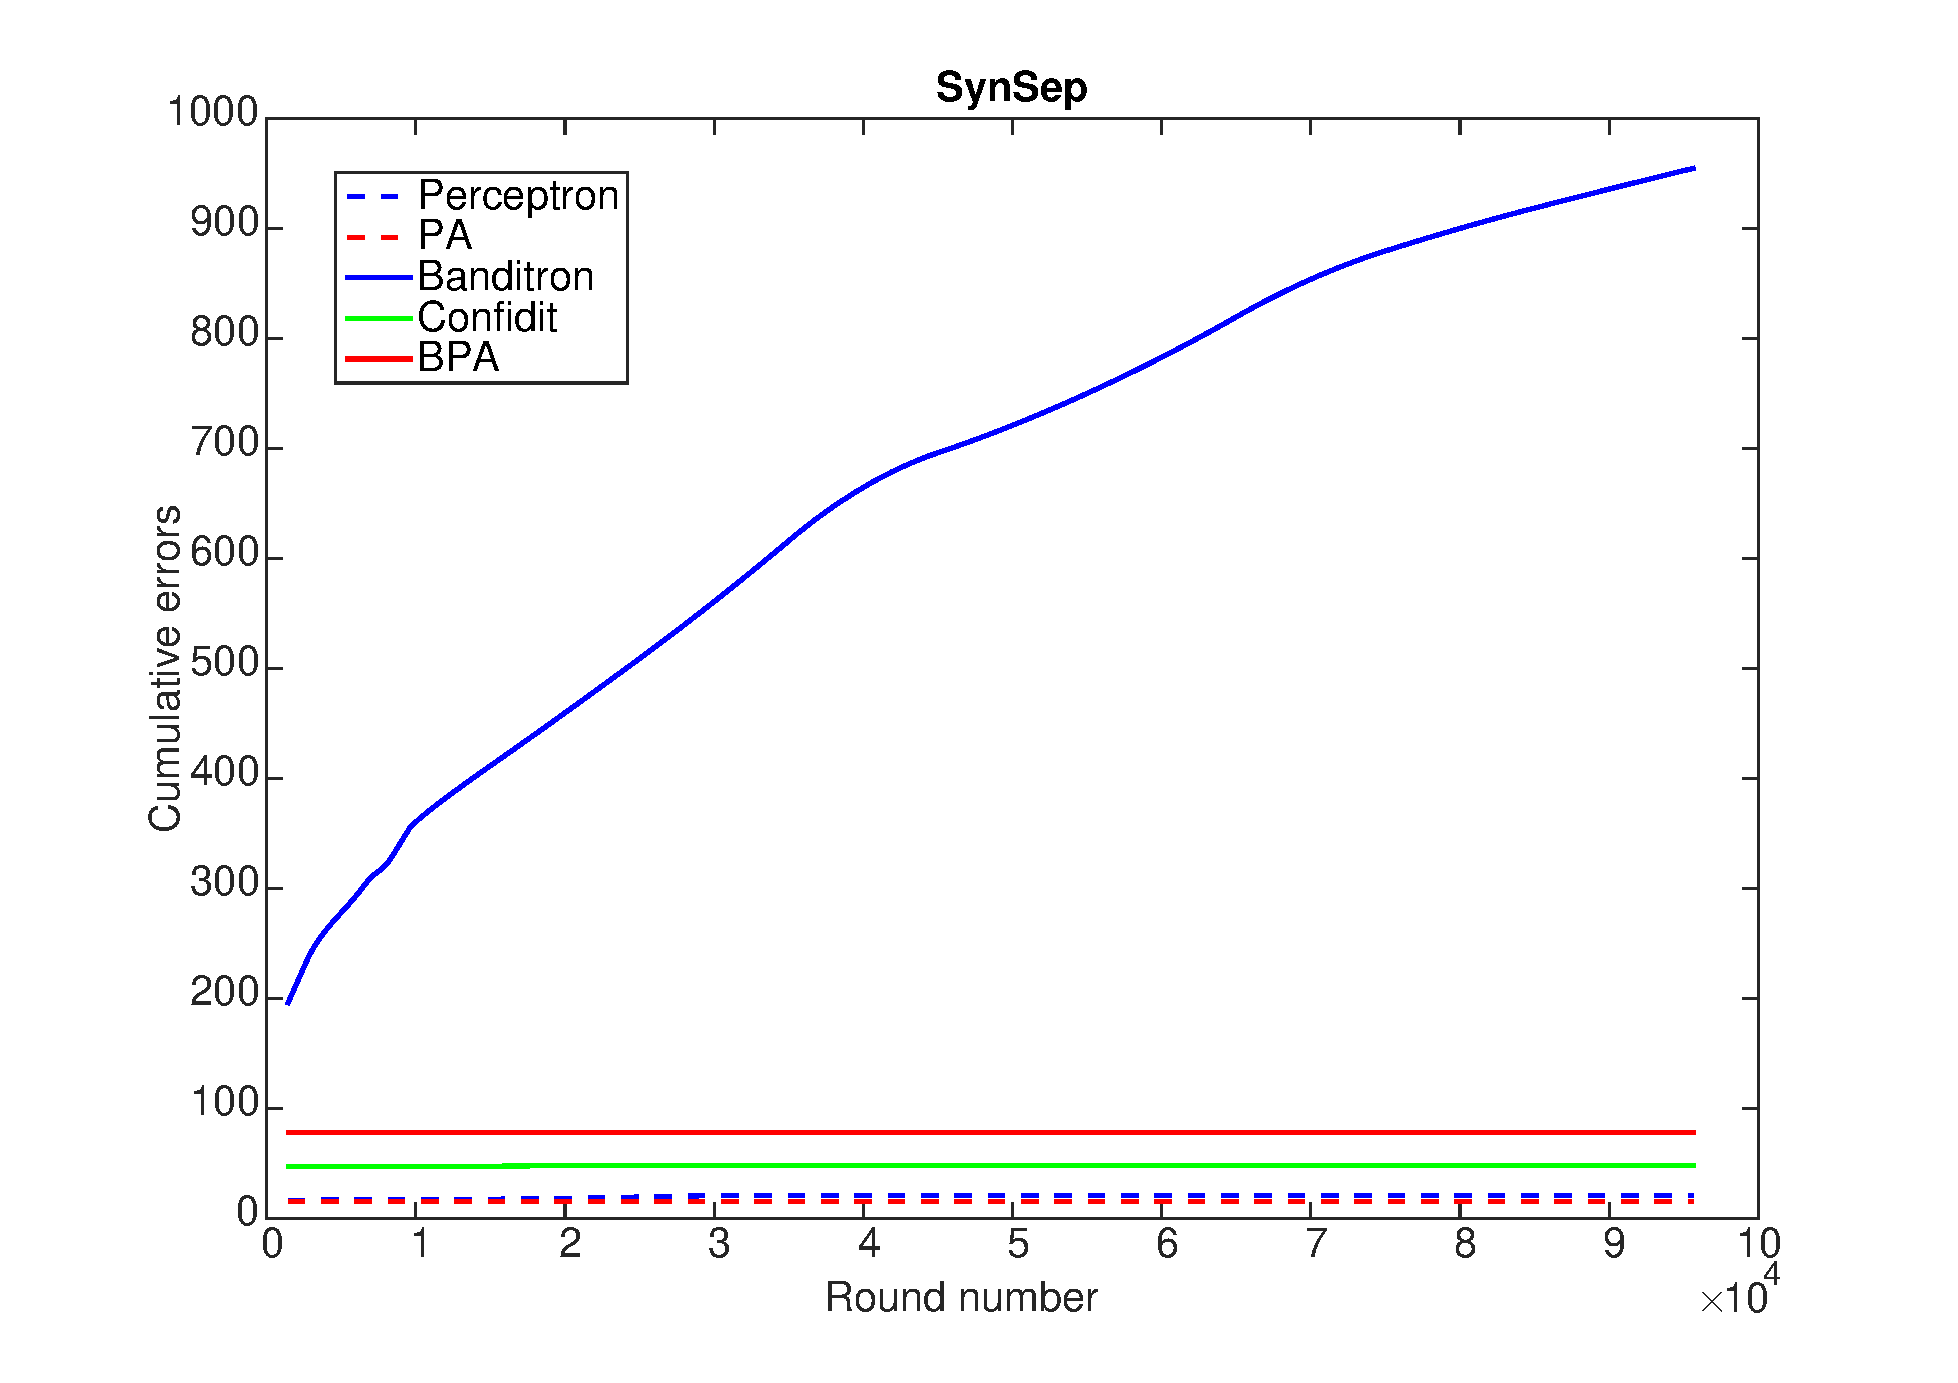
\includegraphics[scale = 0.4]{figs/SynSep.eps}
	}
	\caption{Cumulative Errors on the synthetic data set of  SynSep.}
	\label{pic:BPASS}
\end{figure}
\begin{figure}[h!]
	
	\centerline{
		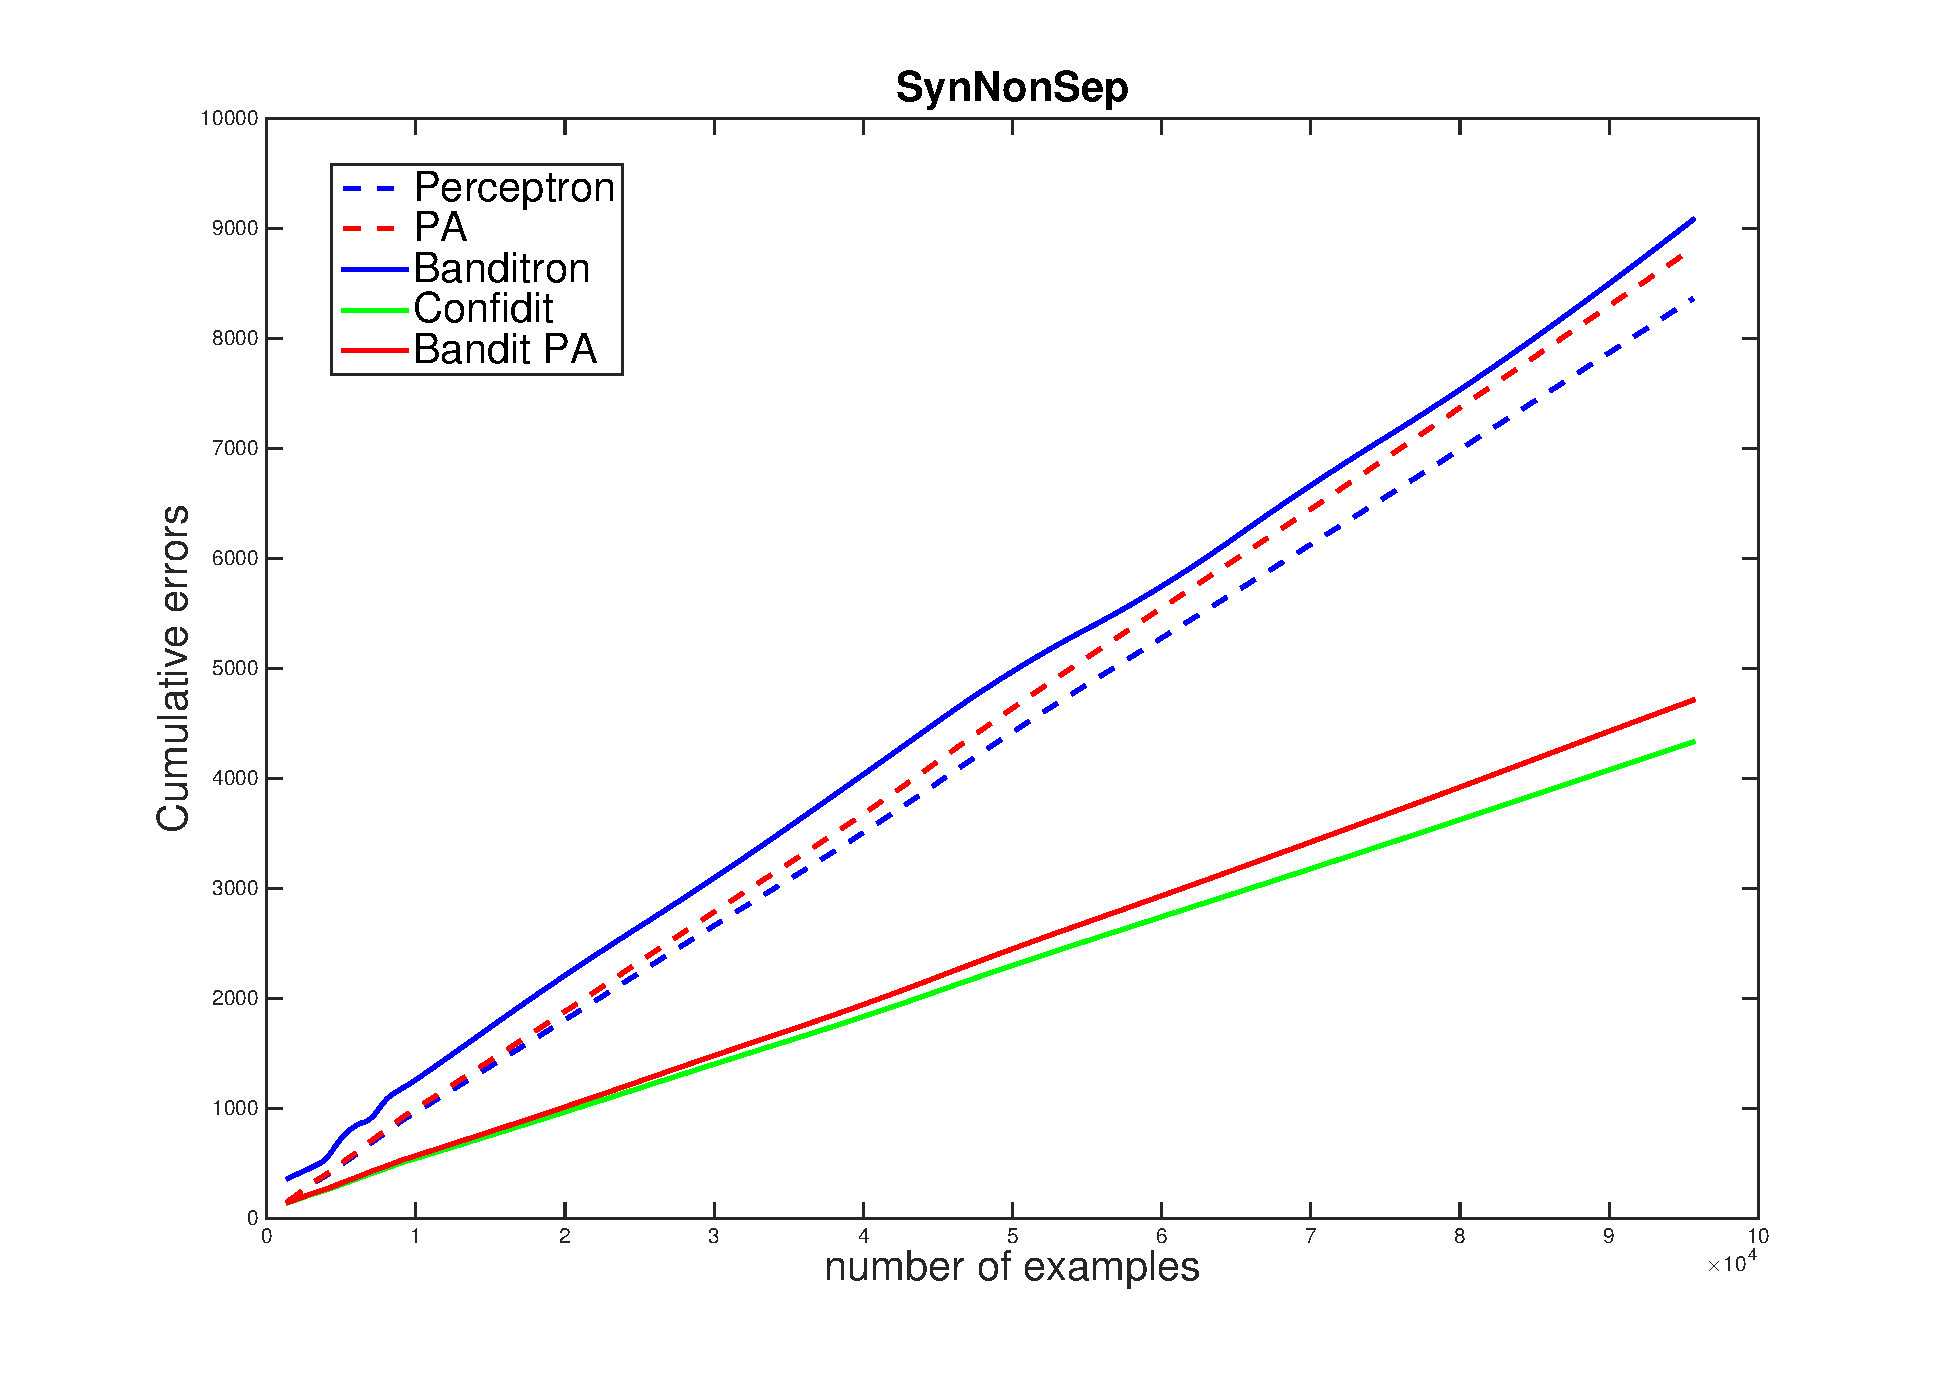
\includegraphics[scale = 0.4]{figs/SynNonSep.eps}
	}
	\caption{Cumulative Errors on the synthetic data set of SynNonSep.}
	\label{pic:BPASNS}
\end{figure}
\begin{figure}[h!]
	\centerline{
		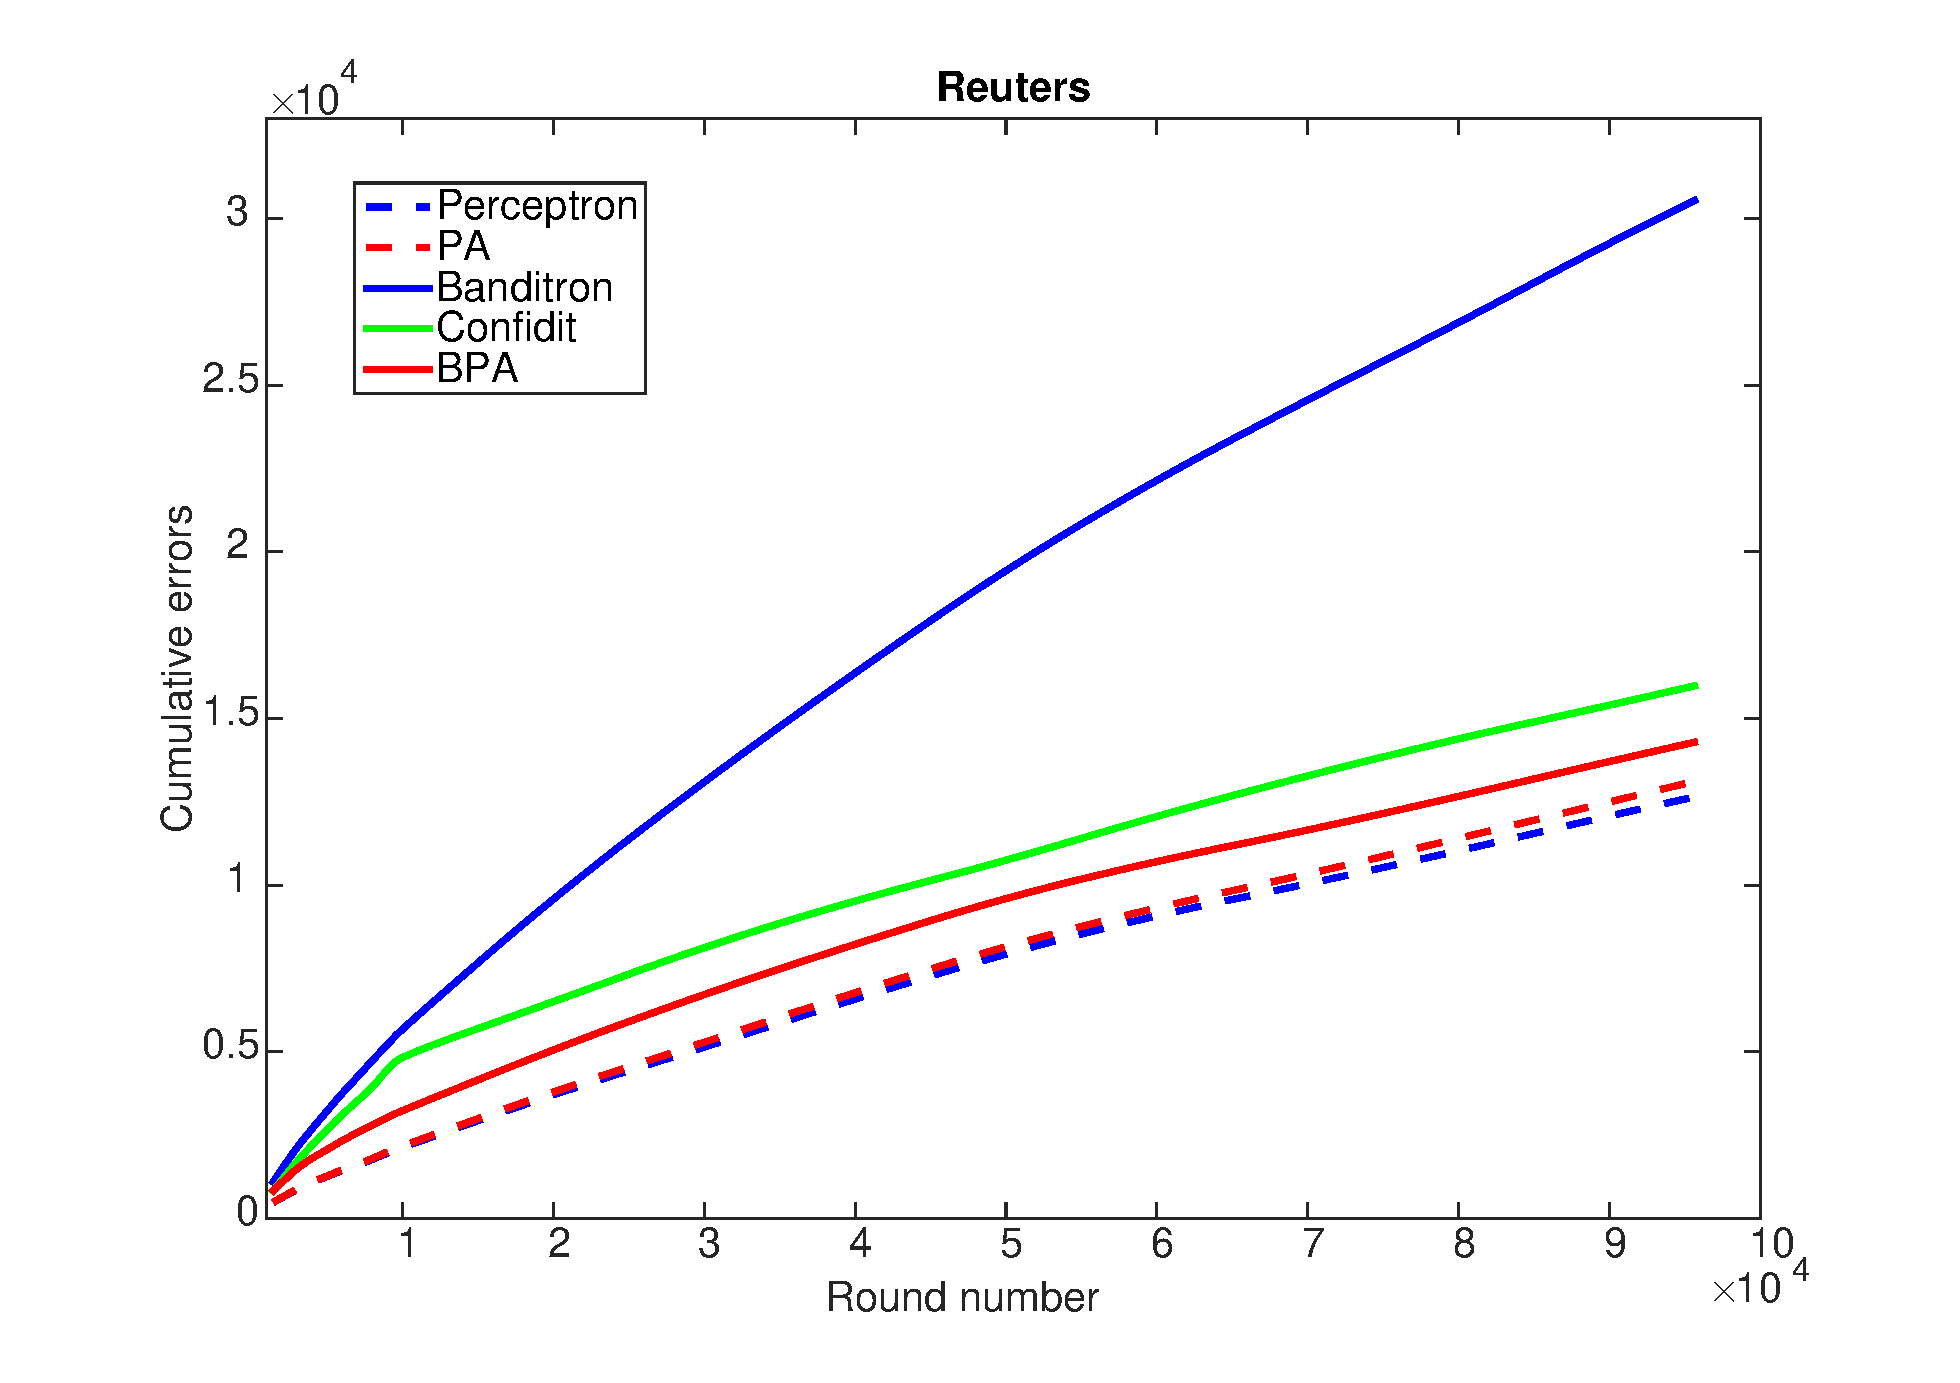
\includegraphics[scale = 0.4]{figs/RCV1_v2_53class.eps}}
	\caption{Cumulative Errors  on the real data set of RCV1-v2 (53 classes).}
	\label{pic:BPARCV}
\end{figure}

\begin{figure}[h!]
	\centerline{
		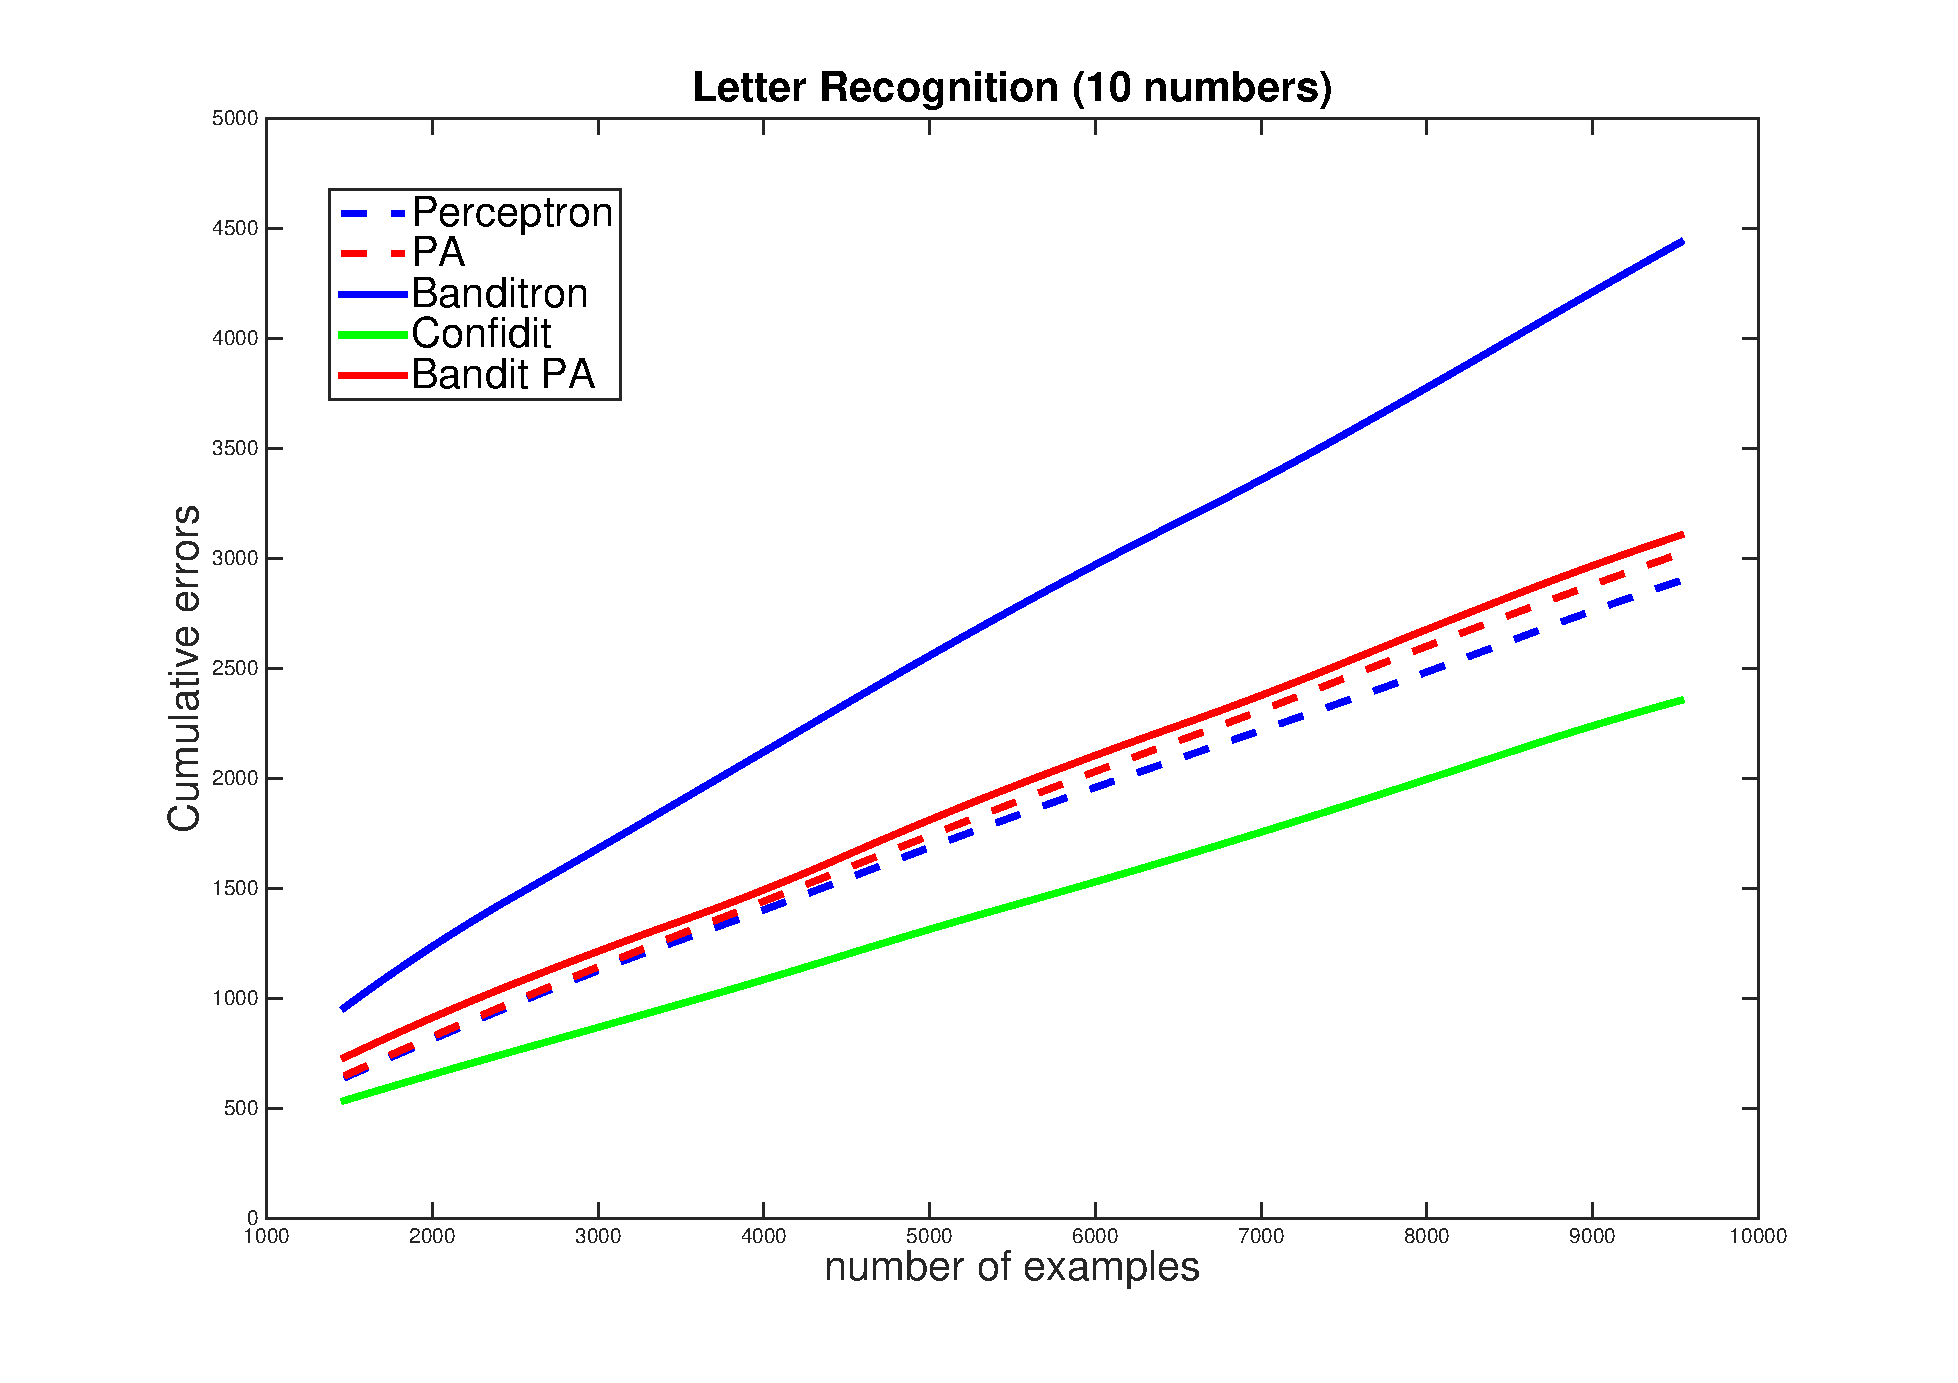
\includegraphics[scale = 0.4]{figs/10LR.eps}}
	\caption{Cumulative Errors on the real data set of Letter Recognition (10 numbers).}
	\label{pic:BPALR10}
\end{figure}

\begin{figure}[h!]
	\centerline{
		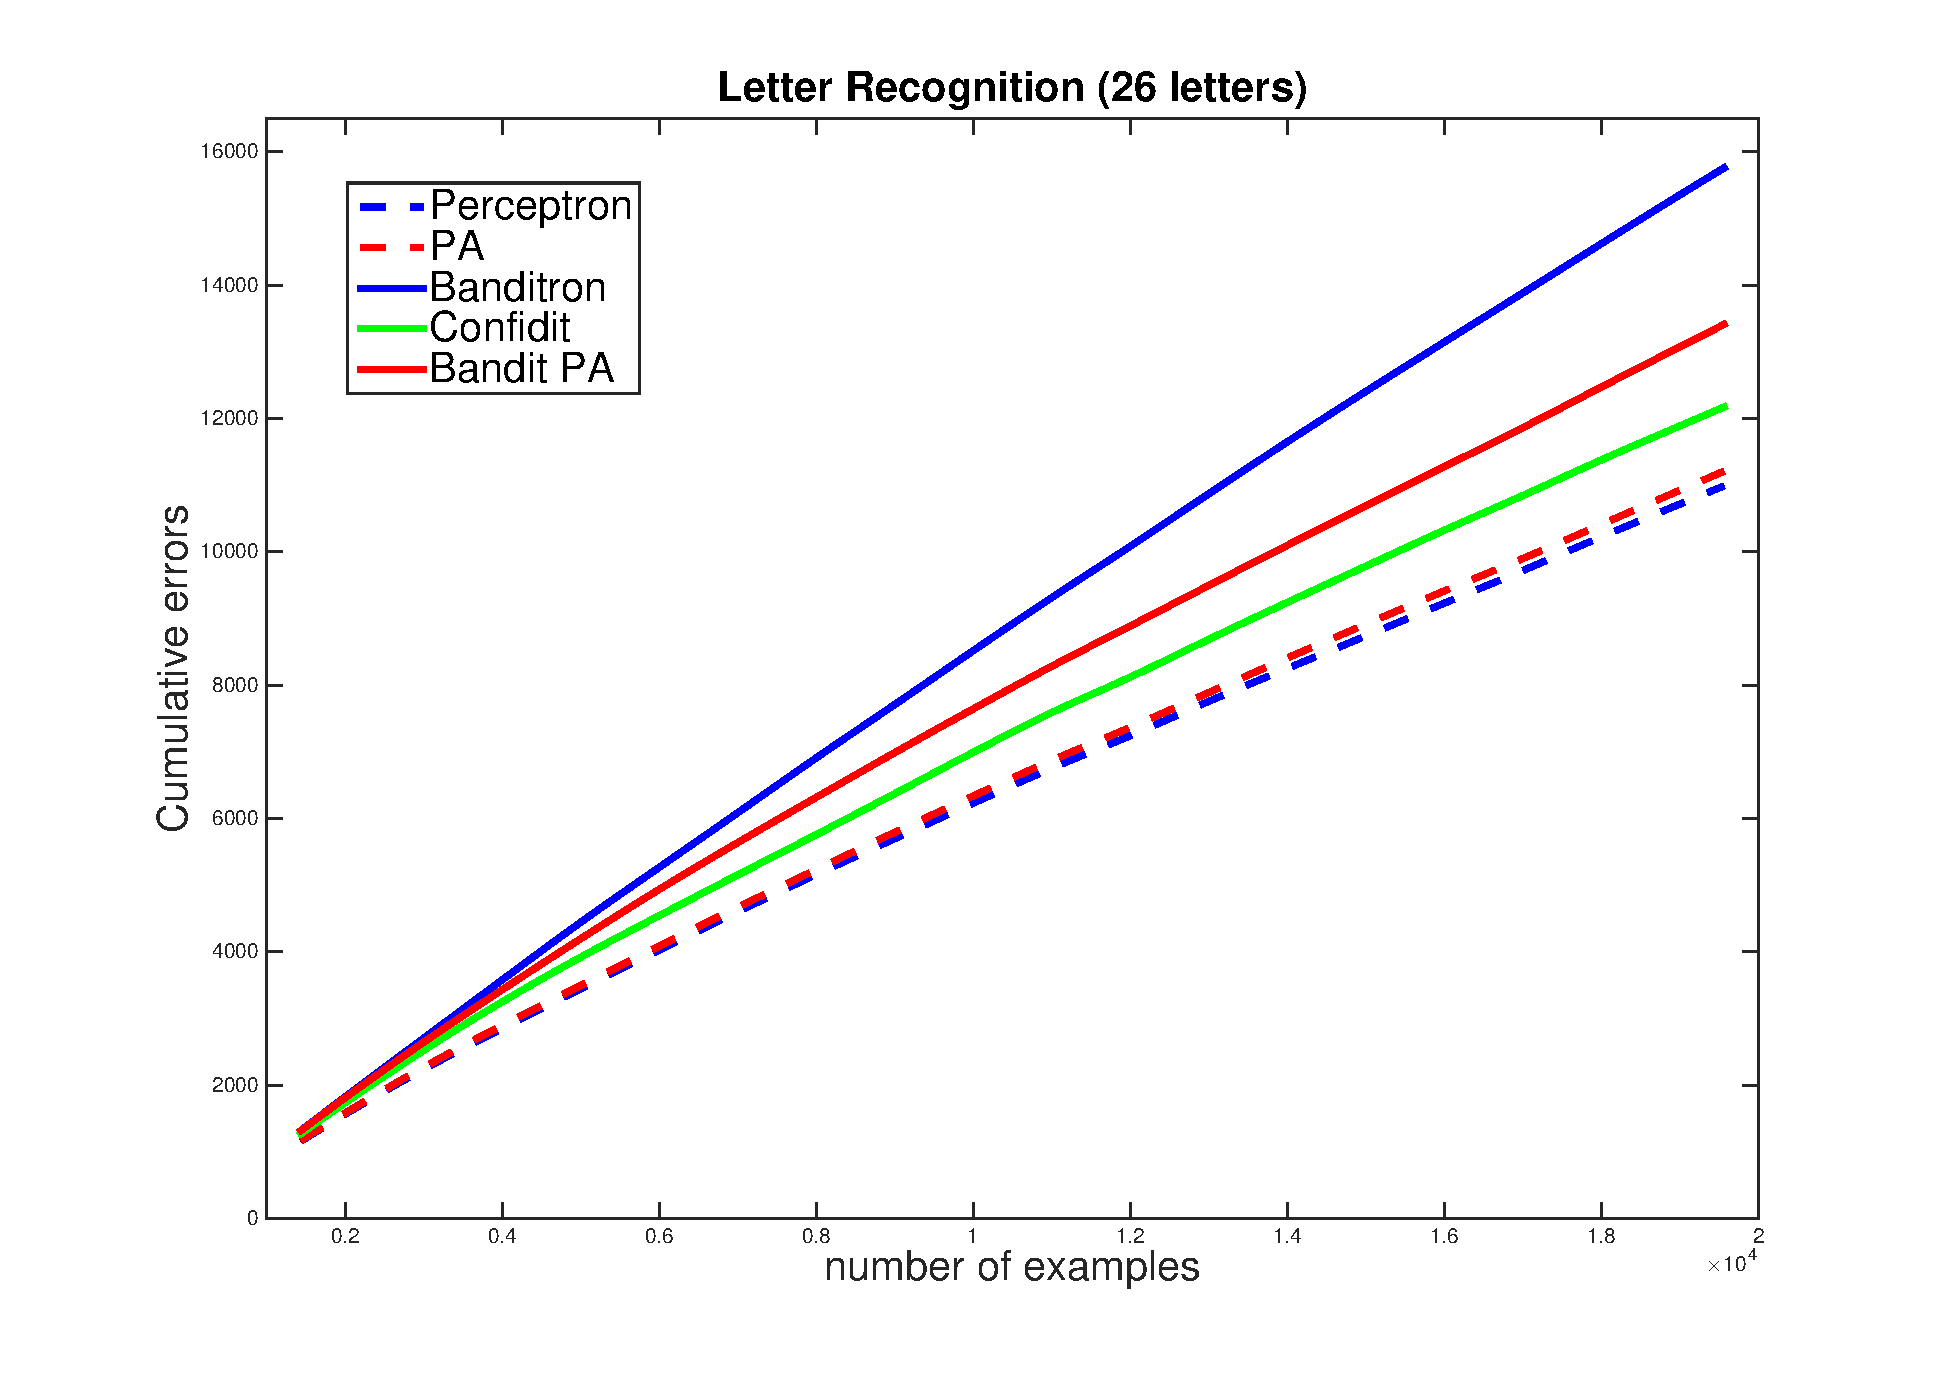
\includegraphics[scale = 0.4]{figs/26LR.eps}}
	\caption{Cumulative Errors  on the real data set of Letter Recognition (26 Letters).}
	\label{pic:BPALR26}
\end{figure}

\begin{figure}[h!]
	\centerline{
		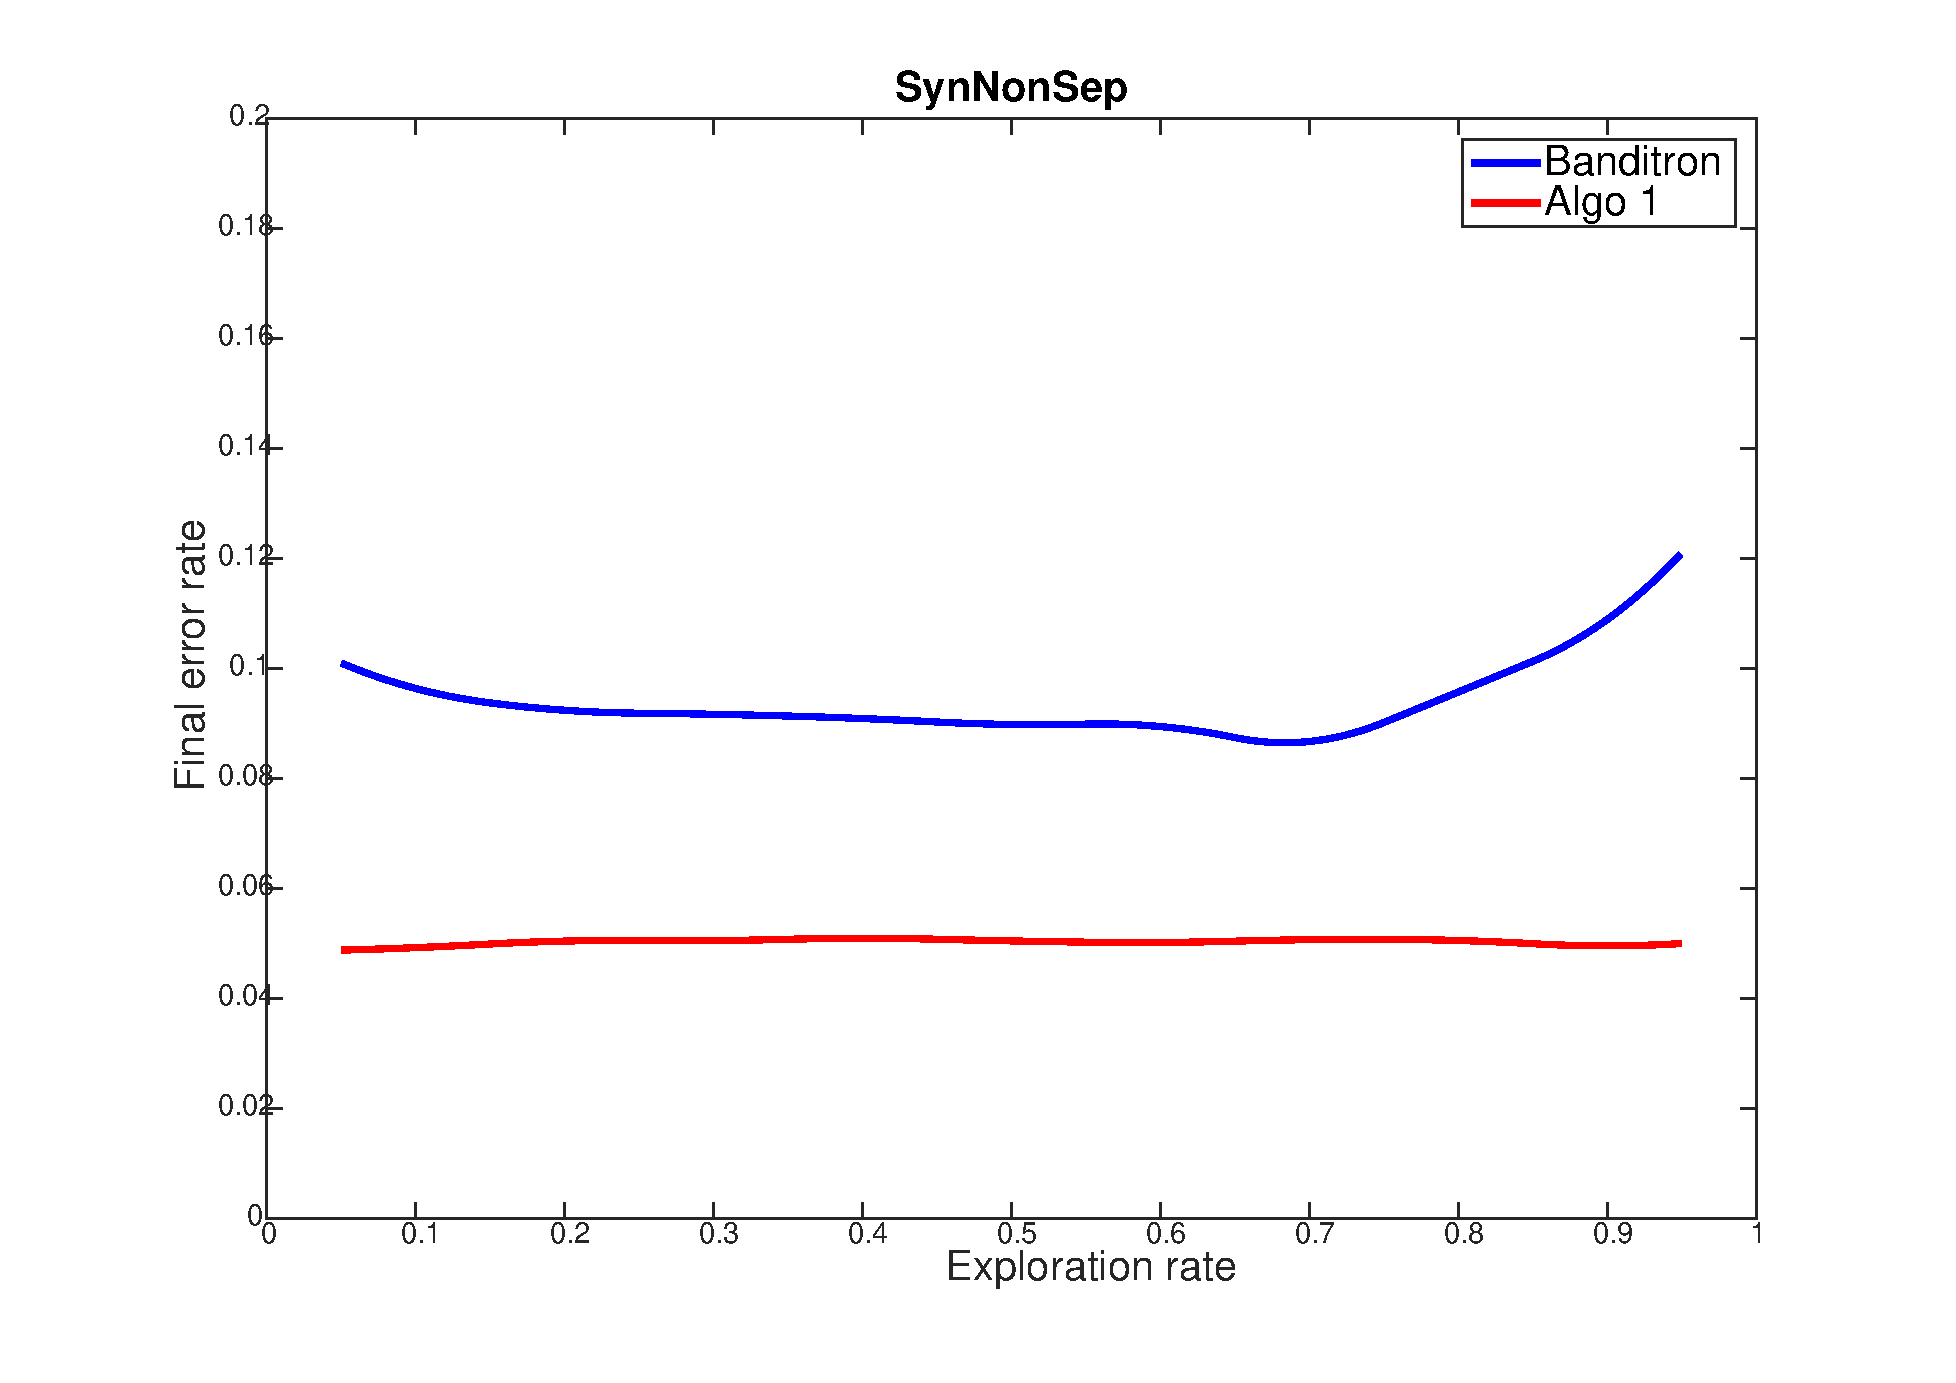
\includegraphics[scale = 0.4]{figs/SynNonSep_gamma.eps}}
	\caption{Average error of Banditron and BPA for parameter's value $\epsilon$ on the data set of SynNonSep. }
	\label{pic:BPASNSerr}
\end{figure}

\begin{figure}[h!]
	\centerline{
		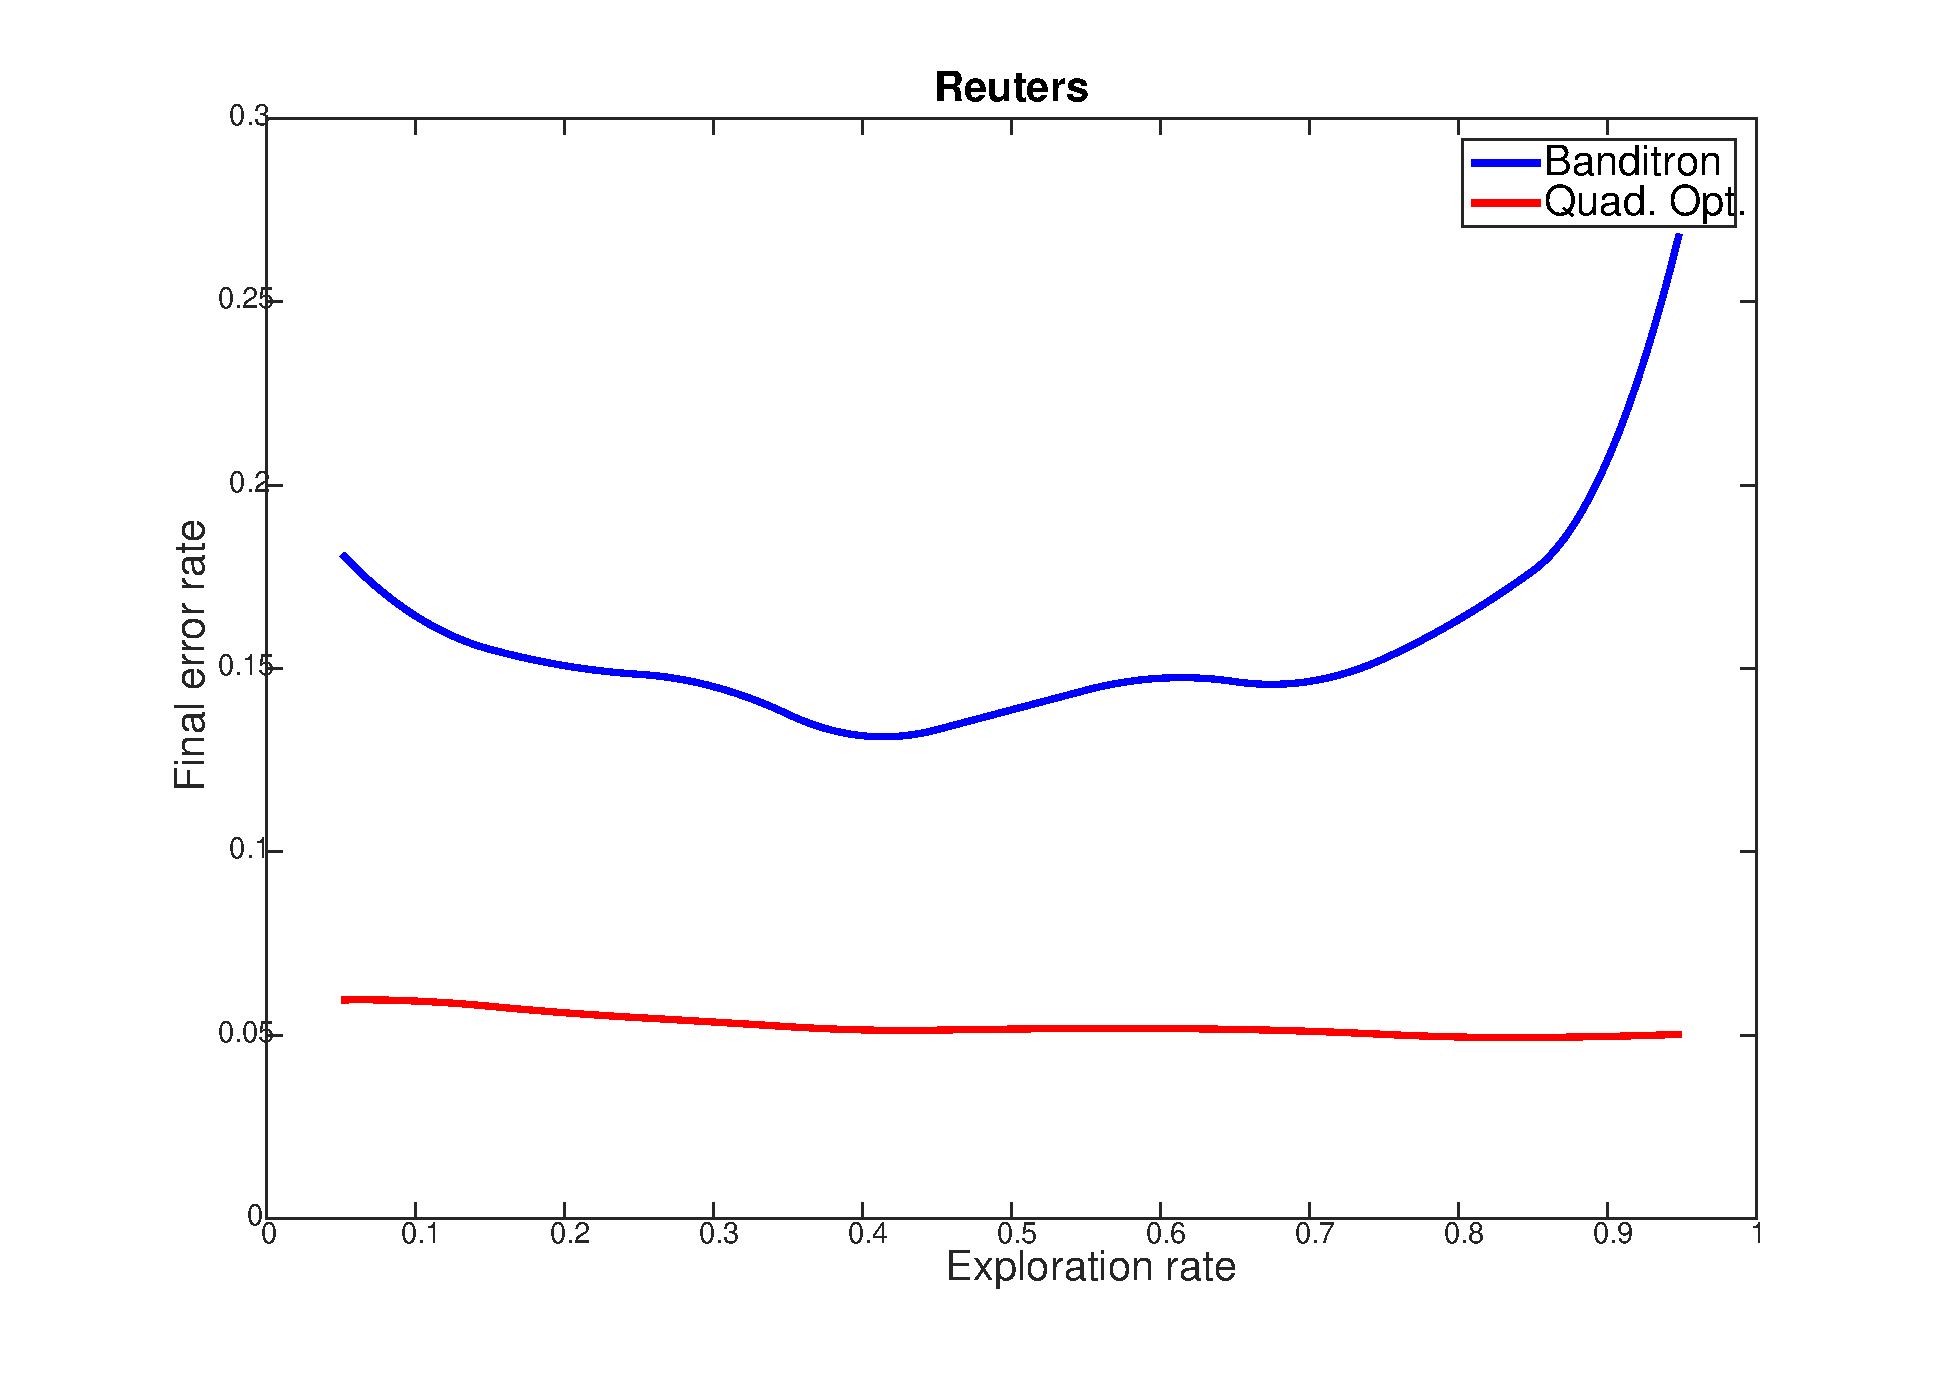
\includegraphics[scale = 0.4]{figs/Reuters_gamma.eps}}
	\caption{Average error of Banditron and BPA for parameter's value $\epsilon$ on the data set of Reuters.}
	\label{pic:BPARCVerr}
\end{figure}

\begin{figure}[h!]
	\centerline{
		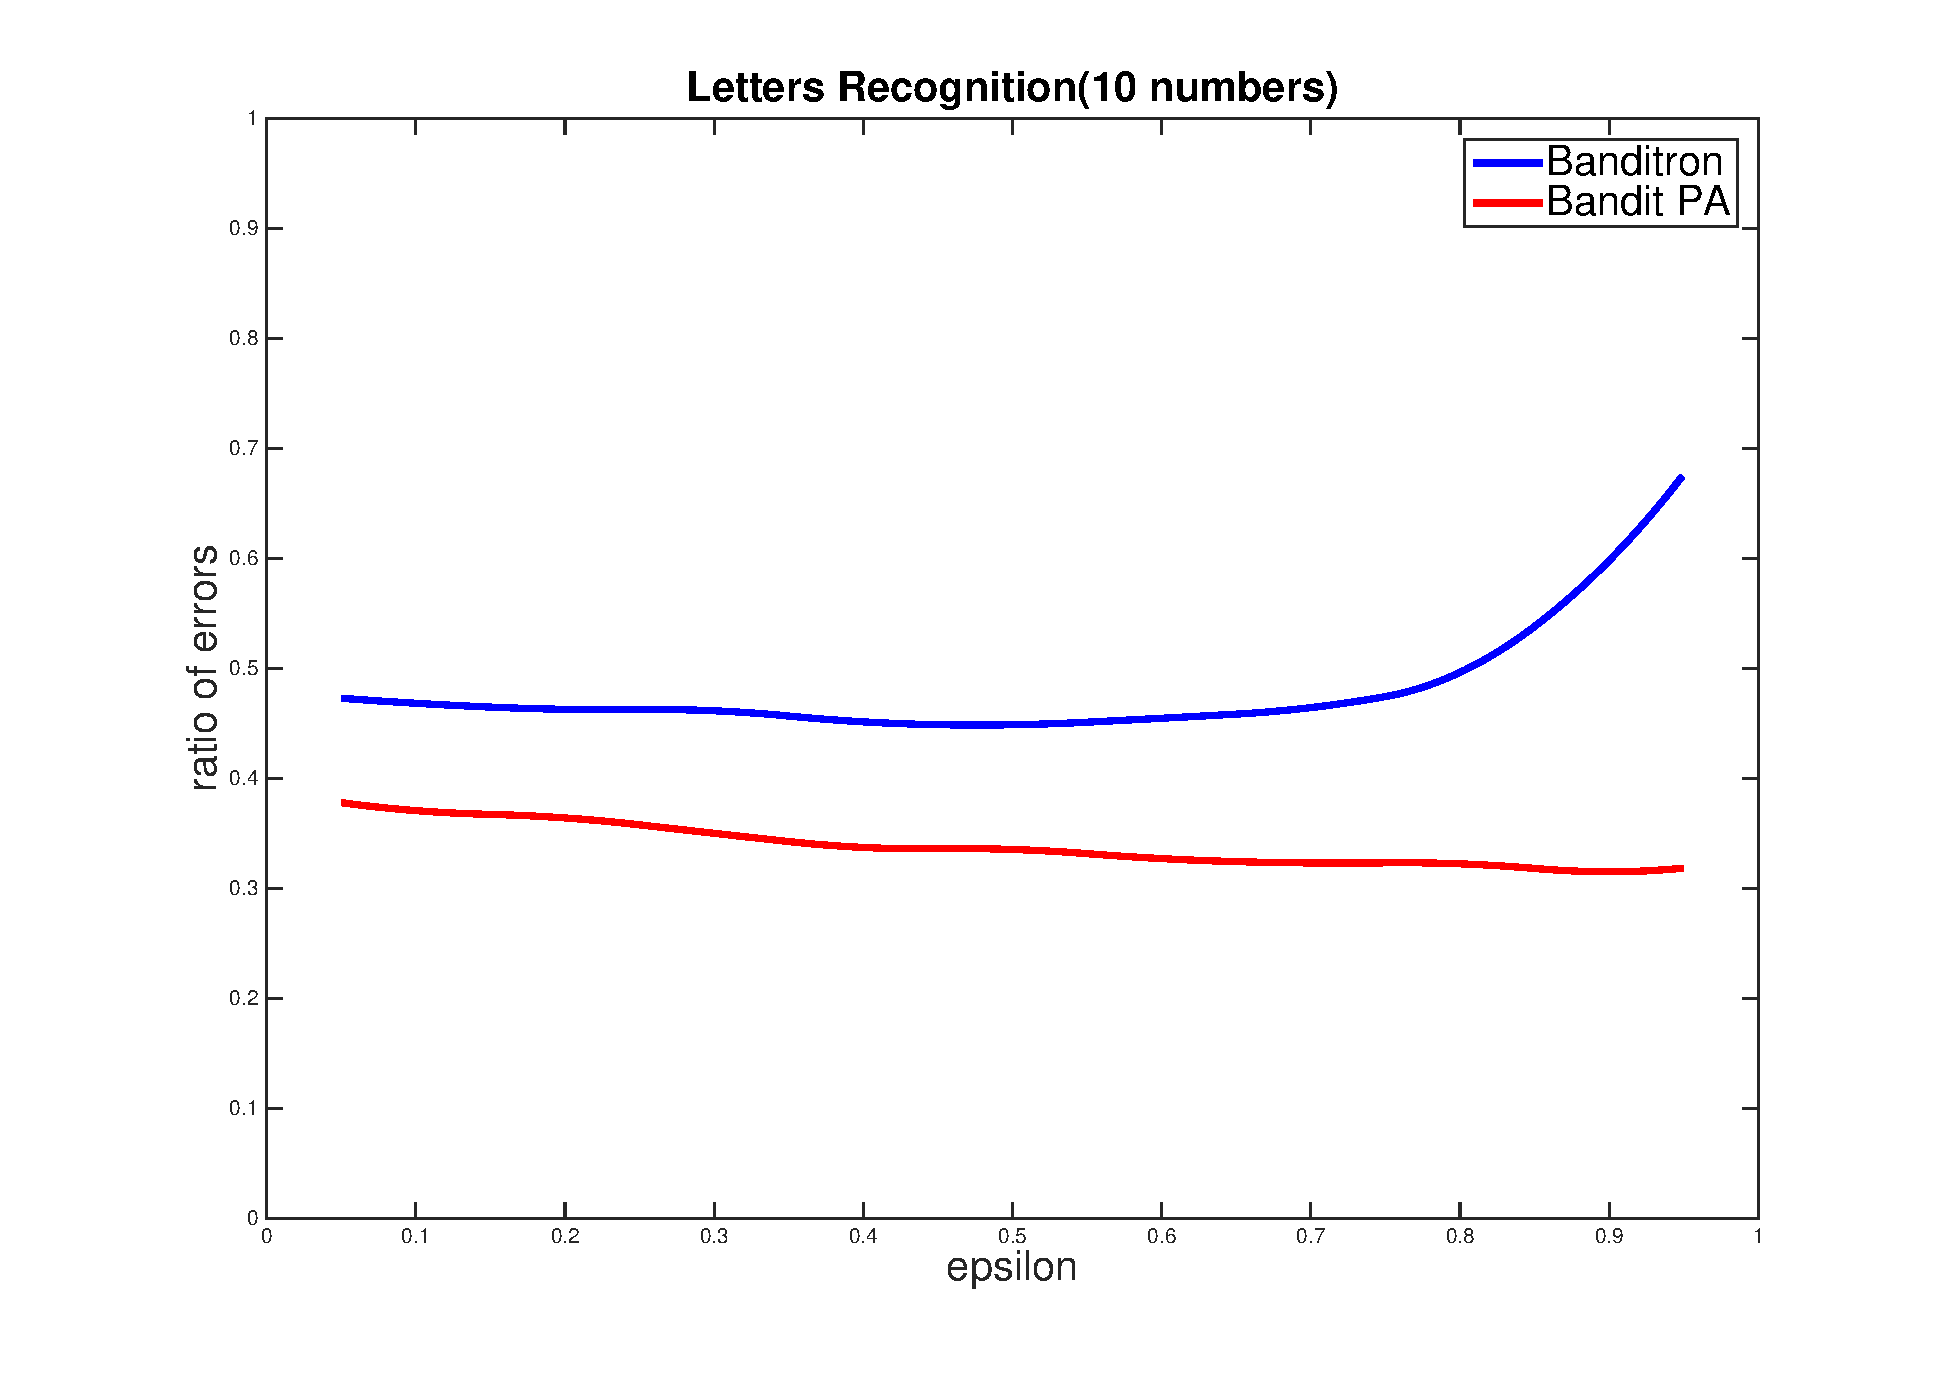
\includegraphics[scale = 0.4]{figs/10LR_gamma.eps}}
	\caption{Average error of Banditron and BPA for parameter's value $\epsilon$ on the data set of Letter Recognition.}
	\label{pic:BPALRerr}
\end{figure}


\subsection{Non-linearly separable datasets}

In this section, we take two datasets to evaluate and analyze the effect of these algorithm in Reproducing Kernel Hilbert Space.

\vspace{1.5ex}
\textbf{Data description}
The first dataset denoted by Pendigits, is a real data and created by E.Alpaydin and Fevzi.Alimoglu \cite{alimoglu1996combining,Alimoglu96methodsof}. 
It  collected 250samples from 44 writers. All writers are asked to write 250 digits in random order inside boxes of 500 by 500 tablet pixel resolution. 
Here, the dataset is part of original one. It contains 7494 instances, 16 features and 10 classes. 

The second dataset denoted by `Segment'\cite{Lichman:2013}. This dataset contains 2310 instances, all of them were drawn randomly from a database of 7 outdoor images. The images were handsegmented to create a clasification for every pixel. Each instance is a $3\times 3$ region. It's a real dataset, with 19 features and 7 classes. More details could be referred to the data site ``UCI''.

\vspace{1.5ex}
%\textcolor{red}{OK-- Il faut donner la formule des noyaux lineaire et Laplace}
\textbf{Algorithm}
Here, we take algorithms Banditron (in RKHS), KBPA and KSGD to compare. In order to perform the effect of RKHS, we choose KBPA in linear model as the reference object and choose \textbf{Laplace} for the kernel function. Its form looks like the following formulate.
\[K_{Laplace}(x,y) = \exp{\left(-\frac{\parallel{x-y}\parallel}{\sigma}\right)}\]
So, all participant algorithms contains: KBanditron, KBPA (linear), KBPA (Laplace), and KSGD (Laplace). For each dataset, the parameter of kernel function is different. By cross-validation way, we choose $\eta = 1$ of model `Laplace' for dataset Pendigits and $\eta = 10$ for dataset `Segment'. For KSGD, the truncated number is 500 for dataset Pendigits, and 200 for Segment.

\vspace{1.5ex}
\textbf{Result}
We mainly analyze these experiments from the following aspects. 

Average training time for each instance:  we observe the training time of every instance $\{t_1,t_2,\dots,t_n\}$; then divide 100 ordering examples into one group $g_1 = \{t_1,\dots,t_{100}\}$,
$\dots$, $g_i = \{t_{1+100*(i-1)},\dots, t_{100*i}\}$; finally, the average training time for instances of group $g_i$ can be calculated by $\overline{t_i} = \frac{1}{100}\sum_{s=1+100*(i-1)}^{100*i} t_s$. 

Average error rate: $e_i = \sum_{s=1+100*(i-1)}^{100\times i}\mathbf{1}_{\hat{y}_t = y_t}/100$ this measure is calculated by the same way.

Cumulative Errors: calculate the total number of past errors.

In Figure~\ref{pic:PKT}, it gives the result of average training time on based dataset ``Pendigits''.  From this result, the training time of three kernel algorithms increases linearly along with the number of training instances. Only the linear model is stable. From the theoretical perspective, Banditron always adds a new example passively for its support vector. Algorithm KSGD only adds a new example for its support vector if its classifier makes a bad prediction, otherwise the number of support vector is limited by the truncated parameter. Algorithm KBPA adds a new example for its support vector if and only if its predicted loss not equals to zero. So its number of support vector will increase all the time until it can make good prediction with no loss.

In Figure~\ref{pic:PKM} and Figure~\ref{pic:PKCM}, accumulative errors of algorithm KBPA firstly tend to a stable, others still increase linearly. That is because KBPA accumulates all good support vectors, KSGD only accumulates several recent support vectors and Kernel Banditron always accumulates new instance as negative support vector.

In Figure~\ref{pic:SKT}, it is about the average training time on dataset ``Segment''.  The training time of Kernel Banditron still increases linearly, while the training time of KSGD and KBPA are as stable as linear model after a small period of increasing linearly. KSGD reaches the limited number of support vector, and KBPA quickly gets enough support vectors to make a good prediction. It could show that this dataset is separable. 

In Figure~\ref{pic:SKM} and Figure~\ref{pic:SKCM}, we can observe that KBPA and KSGD performed obviously better than the other two.  Two kernel algorithms have ability to solve non-linear classification with Bandit Feedback. Considering the scale of classifier, we can use more efficient algorithm KBPA if dataset is separable, otherwise we use KSGD.

\begin{figure}[h!]
	\centerline{
		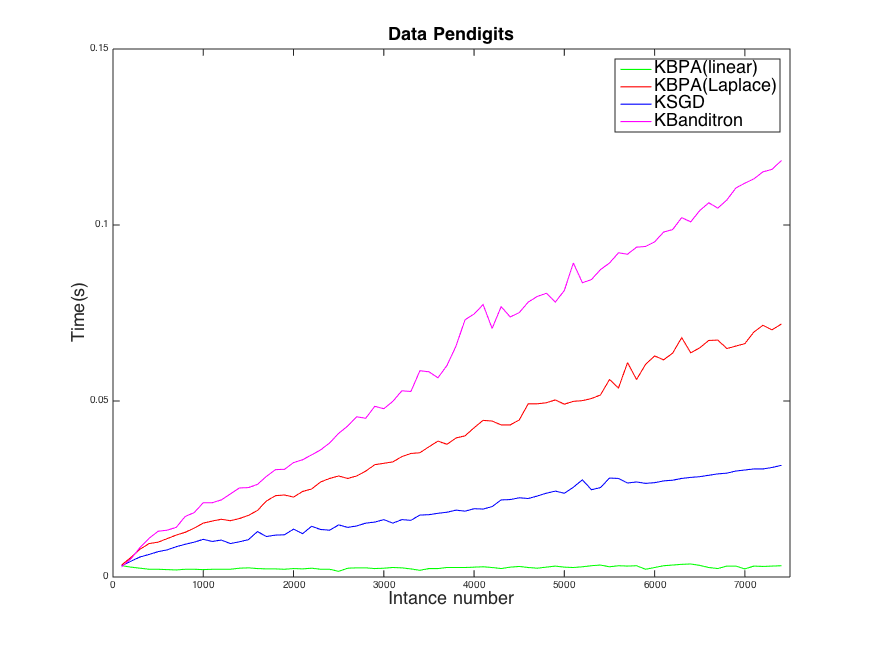
\includegraphics[scale = 0.4]{figs/Pendigits_kernel_T.png}
	}
	\caption{Average training time for each instance of Data Pendigits.}
	\label{pic:PKT}
\end{figure}

\begin{figure}[h!]
	\centerline{
		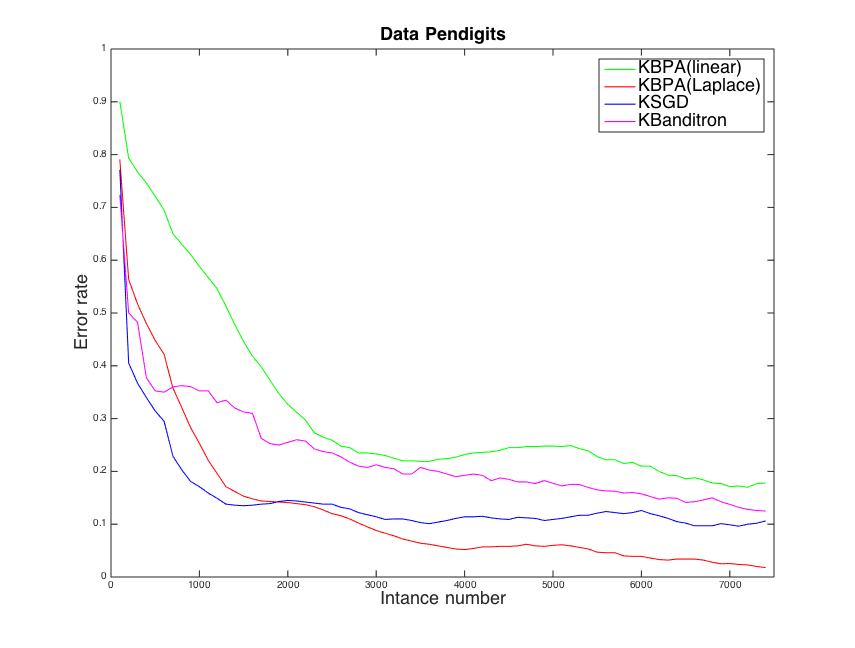
\includegraphics[scale = 0.4]{figs/Pendigits_kernel_M.png}}
	\caption{Average error rate for each instance of Data Pendigits}
	\label{pic:PKM}
\end{figure}

\begin{figure}[h!]
	\centerline{
		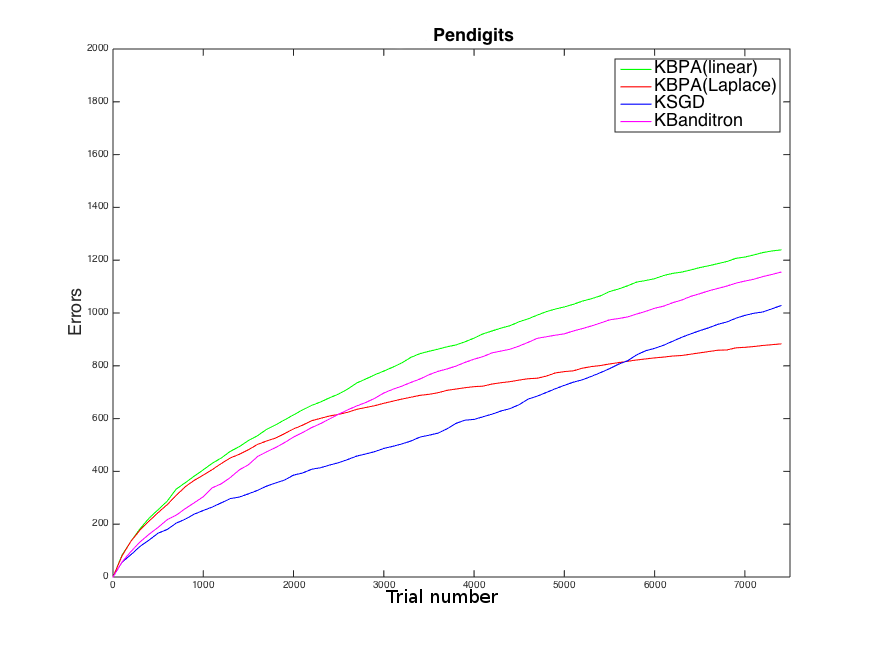
\includegraphics[scale = 0.4]{figs/Pendigits_kernel_CM.png}}
	\caption{Cumulative Errors of Data Pendigits}
	\label{pic:PKCM}
\end{figure}

%\begin{figure}[h!]
%\label{pic:PKR}
%\centerline{
%\includegraphics[scale = 0.4]{fig05/mc/Pendigits_kernel_R.png}}
%\caption{Cumulative loss of Data Pendigits}
%\end{figure}

\begin{figure}[h!]
	\centerline{
		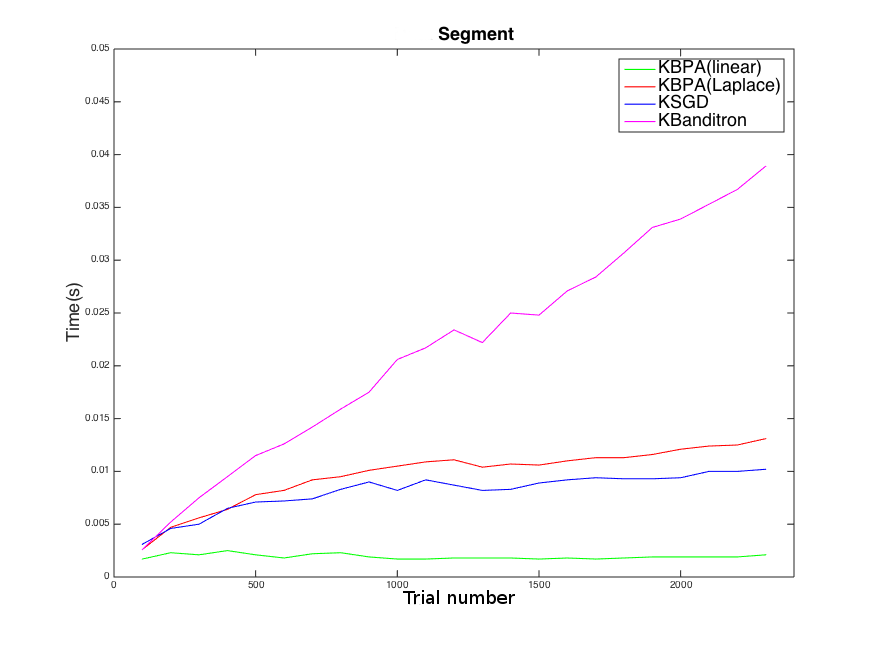
\includegraphics[scale = 0.4]{figs/Segment_kernel_T.png}}
	\caption{Average training time for each instance of Data Segment.}
	\label{pic:SKT}
\end{figure}

\begin{figure}[h!]
	\centerline{
		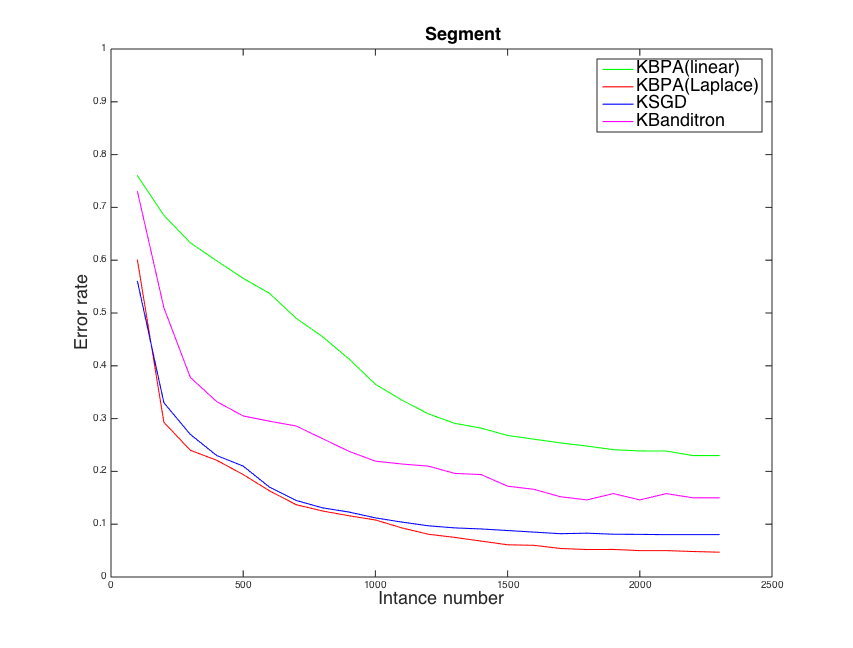
\includegraphics[scale = 0.4]{figs/Segment_kernel_M.png}}
	\caption{Average error rate for each instance of Data Segment}
	\label{pic:SKM}
\end{figure}

\begin{figure}[h!]
	\centerline{
		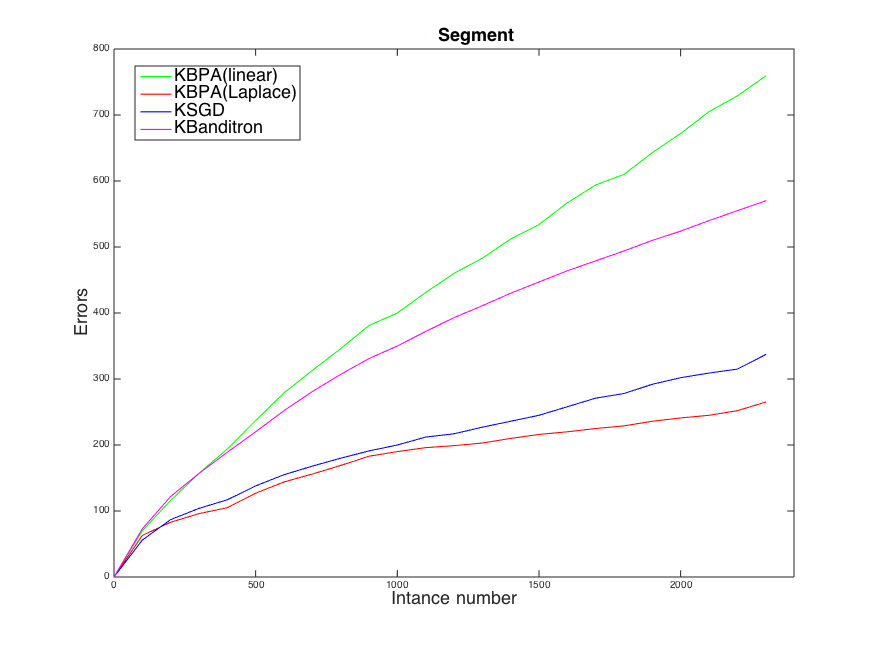
\includegraphics[scale = 0.4]{figs/Segment_kernel_CM.png}}
	\caption{Cumulative Errors of Data Segment}
	\label{pic:SKCM}
\end{figure}

%\begin{figure}[h!]
%\label{pic:SKR}
%\centerline{
%\includegraphics[scale = 0.4]{fig05/mc/Segment_kernel_R.png}}
%\caption{Cumulative loss of Data Segment}
%\end{figure}
%\subsection{Conclusion}
\section{Conclusion}
\label{sec:conclusion}
{Conclusion}
\label{subsec:BPAC}

We proposed a novel algorithm for online multiclass classification with bandit feedback. By the advantage of PA max-margin principle, BPA appears effective to address the bandit online learning setting. Its main advantage is its linear complexity in space that allows to deal with high dimensional data sets and a large number of classes, on the contrary to second-order methods. The practicability of this algorithm is verified theoretically by showing a competitive loss bound.

Moreover, experimental evaluation shows that BPA performs better than other algorithms on  real datasets, even better than the algorithms with full feedback on the data sets non-separable.

%In the next section, we will take BPA to deal with non-linear data sets  by combining the Kernel method. 



%Reading :
%Fundamental Limits of Online and Distributed Algorithms for Statistical Learning and Estimation Ohad Shamir (NIPS’14)
%Many machine learning approaches are characterized by information constraints on how they interact with the training data. These include 
%memory and sequential access constraints (e.g. fast first-order methods to solve stochastic optimization problems); 
%communication constraints (e.g. distributed learning); 
%partial access to the underlying data (e.g. missing features and multi-armed bandits) 
%algorithm with small memory footprint
%The standard implementation of many common learning tasks requires memory which is super-linear in the data dimension
%The need for fast and scalable learning algorithms has popularised the use of online algorithms, which work by sequentially going over the training data, and incrementally updating a (usually small) state vector
%There has also been considerable interest in online learning with partial information, where the learner only gets partial feedback on his performance. This has been used to model various problems in web advertising, routing and multiclass learning. Perhaps the most well-known case is the multi-armed bandits problem with many other variants being developed, such as contextual bandits, combinatorial bandits, and more general models such as partial monitoring [Bubeck, Cesa-Bianchi]
%sequential decisions


%% The Appendices part is started with the command \appendix;
%% appendix sections are then done as normal sections
%% \appendix

%% \section{}
%% \label{}

%% If you have bibdatabase file and want bibtex to generate the
%% bibitems, please use
%%
\bibliographystyle{elsarticle-harv} 
\bibliography{main}

%% else use the following coding to input the bibitems directly in the
%% TeX file.

% %\begin{thebibliography}{00}

%% \bibitem[Author(year)]{label}
%% Text of bibliographic item

%% \bibitem[ ()]{}

% %\end{thebibliography}

\end{document}

\endinput
%%
%% End of file `elsarticle-template-harv.tex'.
